\documentclass[10pt]{article}
\usepackage[T1]{fontenc}
\usepackage[utf8]{inputenc}
% \usepackage{lmodern}
%\usepackage[adobe-utopia,uppercase=upright,greeklowercase=upright]{mathdesign}
\usepackage[adobe-utopia]{mathdesign}
%\usepackage{minionpro}
% \usepackage{pifont}
% \usepackage{amssymb}
\usepackage{amsmath}
\usepackage[francais]{babel}
% \usepackage[francais]{varioref}
\usepackage[dvips]{graphicx}

\usepackage{framed}
\usepackage[normalem]{ulem}
\usepackage{fancyhdr}
\usepackage{titlesec}
\usepackage{vmargin}
\usepackage{longtable}

\usepackage{ifthen}


%\usepackage{epsfig}
\usepackage{subfig}

\usepackage{multirow}
\usepackage{multicol} % Portions de texte en colonnes
\usepackage{flafter}%floatants après la référence



\usepackage{color}
\usepackage{colortbl}


\definecolor{gris25}{gray}{0.75}
\definecolor{bleu}{RGB}{18,33,98}
\definecolor{bleuf}{RGB}{42,94,171}
\definecolor{bleuc}{RGB}{231,239,247}
\definecolor{rougef}{RGB}{185,18,27}
\definecolor{rougec}{RGB}{255,230,231}
\definecolor{vertf}{RGB}{103,126,82}
\definecolor{vertc}{RGB}{220,255,191}

\newenvironment{rem}[1][\hsize]%
{%
    \def\FrameCommand
    {%
\rotatebox{90}{\textit{\textsf{Remarque}}} 
        {\color{bleuf}\vrule width 3pt}%
        \hspace{0pt}%must no space.
        \fboxsep=\FrameSep\colorbox{bleuc}%
    }%
    \MakeFramed{\hsize#1\advance\hsize-\width\FrameRestore}%
}%
{\endMakeFramed}%


\newenvironment{savoir}[1][\hsize]%
{%
    \def\FrameCommand
    {%
\rotatebox{90}{\textit{\textsf{Savoir}}} 
        {\color{bleuf}\vrule width 3pt}%
        \hspace{0pt}%must no space.
        \fboxsep=\FrameSep\colorbox{bleuc}%
    }%
    \MakeFramed{\hsize#1\advance\hsize-\width\FrameRestore}%
}%
{\endMakeFramed}%

\newenvironment{prob}[1][\hsize]%
{%
    \def\FrameCommand%
    {%
\rotatebox{90}{\textit{\textsf{ Problématique}}} 
        {\color{rougef}\vrule width 3pt}%
        \hspace{0pt}%must no space.
        \fboxsep=\FrameSep\colorbox{rougec}%
    }%
    \MakeFramed{\hsize#1\advance\hsize-\width\FrameRestore}%
}%
{\endMakeFramed}%

\newenvironment{obj}[1][\hsize]%
{%
    \def\FrameCommand%
    {%
\rotatebox{90}{\textit{\textsf{ $\;$}}} 
        {\color{rougef}\vrule width 3pt}%
        \hspace{0pt}%must no space.
        \fboxsep=\FrameSep\colorbox{rougec}%
    }%
    \MakeFramed{\hsize#1\advance\hsize-\width\FrameRestore}%
}%
{\endMakeFramed}%

\newenvironment{defi}[1][\hsize]%
{%
    \def\FrameCommand%
    {%
\rotatebox{90}{\textit{\textsf{Définition\\}}} 
        {\color{bleuf}\vrule width 3pt}%
        \hspace{0pt}%must no space.
        \fboxsep=\FrameSep\colorbox{bleuc}%
    }%
    \MakeFramed{\hsize#1\advance\hsize-\width\FrameRestore}%
}%
{\endMakeFramed}%


\newenvironment{hypo}[1][\hsize]%
{%
    \def\FrameCommand%
    {%
\rotatebox{90}{\textit{\textsf{Hypothèse\\}}} 
        {\color{bleuf}\vrule width 3pt}%
        \hspace{0pt}%must no space.
        \fboxsep=\FrameSep\colorbox{bleuc}%
    }%
    \MakeFramed{\hsize#1\advance\hsize-\width\FrameRestore}%
}%
{\endMakeFramed}%


\newenvironment{prop}[1][\hsize]%
{%
    \def\FrameCommand%
    {%
\rotatebox{90}{\textit{\textsf{Propriété\\}}} 
        {\color{bleuf}\vrule width 3pt}%
        \hspace{0pt}%must no space.
        \fboxsep=\FrameSep\colorbox{bleuc}%
    }%
    \MakeFramed{\hsize#1\advance\hsize-\width\FrameRestore}%
}%
{\endMakeFramed}%

\newenvironment{props}[1][\hsize]%
{%
    \def\FrameCommand%
    {%
\rotatebox{90}{\textit{\textsf{Propriétés\\}}} 
        {\color{bleuf}\vrule width 3pt}%
        \hspace{0pt}%must no space.
        \fboxsep=\FrameSep\colorbox{bleuc}%
    }%
    \MakeFramed{\hsize#1\advance\hsize-\width\FrameRestore}%
}%
{\endMakeFramed}%

\newenvironment{exemple}[1][\hsize]%
{%
    \def\FrameCommand%
    {%
\rotatebox{90}{\textit{\textsf{Exemple\\}}} 
        {\color{vertf}\vrule width 3pt}%
        \hspace{0pt}%must no space.
        \fboxsep=\FrameSep\colorbox{vertc}%
    }%
    \MakeFramed{\hsize#1\advance\hsize-\width\FrameRestore}%
}%
{\endMakeFramed}%

\newenvironment{resultat}[1][\hsize]%
{%
    \def\FrameCommand%
    {%
\rotatebox{90}{\textit{\textsf{Résultat\\}}} 
        {\color{rougef}\vrule width 3pt}%
        \hspace{0pt}%must no space.
        \fboxsep=\FrameSep\colorbox{rougec}%
    }%
    \MakeFramed{\hsize#1\advance\hsize-\width\FrameRestore}%
}%
{\endMakeFramed}%

\newenvironment{methode}[1][\hsize]%
{%
    \def\FrameCommand%
    {%
\rotatebox{90}{\textit{\textsf{Méthode\\}}} 
        {\color{rougef}\vrule width 3pt}%
        \hspace{0pt}%must no space.
        \fboxsep=\FrameSep\colorbox{rougec}%
    }%
    \MakeFramed{\hsize#1\advance\hsize-\width\FrameRestore}%
}%
{\endMakeFramed}%

\newenvironment{theo}[1][\hsize]%
{%
    \def\FrameCommand%
    {%
\rotatebox{90}{\textit{\textsf{Théorème\\}}} 
        {\color{rougef}\vrule width 3pt}%
        \hspace{0pt}%must no space.
        \fboxsep=\FrameSep\colorbox{rougec}%
    }%
    \MakeFramed{\hsize#1\advance\hsize-\width\FrameRestore}%
}%
{\endMakeFramed}%

\newenvironment{warn}[1][\hsize]%
{%
    \def\FrameCommand%
    {%
\rotatebox{90}{\textit{\textsf{Attention\\}}} 
        {\color{rougef}\vrule width 3pt}%
        \hspace{0pt}%must no space.
        \fboxsep=\FrameSep\colorbox{rougec}%
    }%
    \MakeFramed{\hsize#1\advance\hsize-\width\FrameRestore}%
}%
{\endMakeFramed}%

% \usepackage{pstricks}
%\usepackage{minitoc}
% \setcounter{minitocdepth}{4}

\setcounter{tocdepth}{2}

% \mtcselectlanguage{french} 

%\usepackage{draftcopy}% "Brouillon"
% \usepackage{floatflt}
\usepackage{psfrag}
%\usepackage{listings} % Permet d'insérer du code de programmation
\renewcommand{\baselinestretch}{1.2}

% Changer la numérotation des figures :
% ------------------------------------
% \makeatletter
% \renewcommand{\thefigure}{\ifnum \c@section>\z@ \thesection.\fi
%  \@arabic\c@figure}
% \@addtoreset{figure}{section}
% \makeatother
 


%%%%%%%%%%%%
% Définition des vecteurs %
%%%%%%%%%%%%
 \newcommand{\vect}[1]{\overrightarrow{#1}}

%%%%%%%%%%%%
% Définition des torseusr %
%%%%%%%%%%%%

 \newcommand{\torseur}[1]{%
\left\{{#1}\right\}
}

\newcommand{\torseurcin}[3]{%
\left\{\mathcal{#1} \left(#2/#3 \right) \right\}
}

\newcommand{\torseurstat}[3]{%
\left\{\mathcal{#1} \left(#2\rightarrow #3 \right) \right\}
}

 \newcommand{\torseurc}[8]{%
%\left\{#1 \right\}=
\left\{
{#1}
\right\}
 = 
\left\{%
\begin{array}{cc}%
{#2} & {#5}\\%
{#3} & {#6}\\%
{#4} & {#7}\\%
\end{array}%
\right\}_{#8}%
}

 \newcommand{\torseurcol}[7]{
\left\{%
\begin{array}{cc}%
{#1} & {#4}\\%
{#2} & {#5}\\%
{#3} & {#6}\\%
\end{array}%
\right\}_{#7}%
}

 \newcommand{\torseurl}[3]{%
%\left\{\mathcal{#1}\right\}_{#2}=%
\left\{%
\begin{array}{l}%
{#1} \\%
{#2} %
\end{array}%
\right\}_{#3}%
}

 \newcommand{\vectv}[3]{%
\vect{V\left( {#1} \in {#2}/{#3}\right)}
}


\newcommand{\vectf}[2]{%
\vect{R\left( {#1} \rightarrow {#2}\right)}
}

\newcommand{\vectm}[3]{%
\vect{\mathcal{M}\left( {#1}, {#2} \rightarrow {#3}\right)}
}


 \newcommand{\vectg}[3]{%
\vect{\Gamma \left( {#1} \in {#2}/{#3}\right)}
}

 \newcommand{\vecto}[2]{%
\vect{\Omega\left( {#1}/{#2}\right)}
}
% }$$\left\{\mathcal{#1} \right\}_{#2} =%
% \left\{%
% \begin{array}{c}%
%  #3 \\%
%  #4 %
% \end{array}%
% \right\}_{#5}}

%  ------------------------------------------
% | Modification du formatage des sections : | 
%  ------------------------------------------

% Grands titres :
% ---------------

\newcommand{\titre}[1]{%
\begin{center}
      \bigskip
      \rule{\textwidth}{1pt}
      \par\vspace{0.1cm}
      
      \textbf{\large #1}
      \par\rule{\textwidth}{1pt}
    \end{center}
    \bigskip
  }

% Supprime le numéro du chapitre dans la numérotation des sections:
% -----------------------------------------------------------------
\makeatletter
\renewcommand{\thesection}{\@arabic\c@section}
\makeatother


% \titleformat{\chapter}[display]
% {\normalfont\Large\filcenter}
% {}
% {1pc}
% {\titlerule[1pt]
%   \vspace{1pc}%
%   \Huge}[\vspace{1ex}%
% \titlerule]


%%%% Chapitres Comme PY Pechard %%%%%%%%%
% numéro du chapitre
\DeclareFixedFont{\chapnumfont}{OT1}{phv}{b}{n}{80pt}
% pour le mot « Chapitre »
\DeclareFixedFont{\chapchapfont}{OT1}{phv}{m}{it}{40pt}
% pour le titre
\DeclareFixedFont{\chaptitfont}{T1}{phv}{b}{n}{25pt}

\definecolor{gris}{gray}{0.75}
\titleformat{\chapter}[display]%
	{\sffamily}%
	{\filleft\chapchapfont\color{gris}\chaptertitlename\
	\\
	\vspace{12pt}
	\chapnumfont\thechapter}%
	{16pt}%
	{\filleft\chaptitfont}%
	[\vspace{6pt}\titlerule\titlerule\titlerule]

%%%%  Fin Chapitres Comme PY Pechard %%%%%%%%%


% Section, subsection, subsubsection sans serifs :
% % ----------------------------------------------

% \makeatletter
% \renewcommand{\section}{\@startsection{section}{0}{0mm}%
% {\baselineskip}{.3\baselineskip}%
% {\normalfont\sffamily\Large\textbf}}%
% \makeatother

\makeatletter
\renewcommand{\@seccntformat}[1]{{\textcolor{bleu}{\csname
the#1\endcsname}\hspace{0.5em}}}
\makeatother

\makeatletter
\renewcommand{\section}{\@startsection{section}{1}{\z@}%
                       {-4ex \@plus -1ex \@minus -.4ex}%
                       {1ex \@plus.2ex }%
                       {\normalfont\Large\sffamily\bfseries}}%
\makeatother
 
\makeatletter
\renewcommand{\subsection}{\@startsection {subsection}{2}{\z@}
                          {-3ex \@plus -0.1ex \@minus -.4ex}%
                          {0.5ex \@plus.2ex }%
                          {\normalfont\large\sffamily\bfseries}}
\makeatother
 
\makeatletter
\renewcommand{\subsubsection}{\@startsection {subsubsection}{3}{\z@}
                          {-2ex \@plus -0.1ex \@minus -.2ex}%
                          {0.2ex \@plus.2ex }%
                          {\normalfont\large\sffamily\bfseries}}
\makeatother
 
\makeatletter             
\renewcommand{\paragraph}{\@startsection{paragraph}{4}{\z@}%
                                    {-2ex \@plus-.2ex \@minus .2ex}%
                                    {0.1ex}%               
{\normalfont\sffamily\bfseries}}
\makeatother
 
\makeatletter
\renewcommand{\subparagraph}{\@startsection{subparagraph}{5}{\z@}%
                                       {-2ex \@plus-.1ex \@minus .2ex}%
                                       {0.1ex}%
				    {\normalfont\normalsize\sffamily\bfseries}}
\makeatletter
% \makeatletter
% \renewcommand{\subsection}{\@startsection{subsection}{1}{2mm}%
% {\baselineskip}{.3\baselineskip}%
% {\normalfont\sffamily\large\textbf}}%
% \makeatother
% 
% \makeatletter
% \renewcommand{\subsubsection}{\@startsection{subsubsection}{2}{4mm}%
% {\baselineskip}{.15\baselineskip}%
% {\normalfont\sffamily\large\textbf}}%
% \makeatother
% 
% \makeatletter
% \renewcommand{\paragraph}{\@startsection{paragraph}{3}{6mm}%
% {\baselineskip}{.15\baselineskip}%
% {\normalfont\sffamily\large\textbf}}%
% \makeatother
 
\setcounter{secnumdepth}{4}


%  --------
% | Marges |
%  --------


% \setmarginsrb{2.5cm}{1.5cm}{2.5cm}{2cm}{1cm}{1cm}{1cm}{1cm}
\setmarginsrb{1.5cm}{1cm}{1cm}{1.5cm}{1cm}{1cm}{1cm}{1cm}

% Changer les marges localement :
% -----------------------------
\newenvironment{changemargin}[2]{\begin{list}{}{%
\setlength{\topsep}{0pt}%
\setlength{\leftmargin}{0pt}%
\setlength{\rightmargin}{0pt}%
\setlength{\listparindent}{\parindent}%
\setlength{\itemindent}{\parindent}%
\setlength{\parsep}{0pt plus 1pt}%
\addtolength{\leftmargin}{#1}%
\addtolength{\rightmargin}{#2}%
}\item }{\end{list}}



\usepackage{pst-solides3d}
\usepackage{titletoc}
\titlecontents{chapter}[+3pc]
  {\addvspace{10pt}\sffamily\bfseries}
{\contentslabel[{\pscirclebox[fillstyle=solid,fillcolor=gray!25,
linecolor=gray!25,framesep=4pt]{\textcolor{white}{\thecontentslabel}}}]{2.5pc}}
  {}
  {\dotfill \normalfont\thecontentspage\ }

\titlecontents{section}[3pc]
  {\addvspace{2pt}\sffamily}
  {\contentslabel[\thecontentslabel]{1.8pc}}
  {}
  {\dotfill \normalfont\thecontentspage\ }

\titlecontents{subsection}[5pc]
  {\addvspace{2pt}\sffamily}
  {\contentslabel[\thecontentslabel]{1.8pc}}
  {}
  {\dotfill \normalfont\thecontentspage\ }

\titlecontents{subsubsection}[8pc]
  {\addvspace{2pt}\sffamily}
  {\contentslabel[\thecontentslabel]{3pc}}
  {}
  {\dotfill \normalfont\thecontentspage\ }
%{\;\titlerule\;\normalfont\thecontentspage\ }

\titlecontents{paragraph}[9pc]
  {\addvspace{2pt}\sffamily}
  {\contentslabel[\thecontentslabel]{3.5pc}}
  {}
  {\dotfill \normalfont\thecontentspage\ }



%\usepackage{algorithm}
%\usepackage{algorithmic}
\usepackage[french]{algorithm2e}

\SetKwBlock{Fonction}{Début Fonction}{Fin Fonction}
\SetKwComment{Comment}{start}{end}
% Python sources

\usepackage{listings}
\lstloadlanguages{R}   % pour regler les pb d accent utf8 dans les codes
\lstset{language=R} % pour regler les pb d accent utf8 dans les codes

\usepackage{textcomp}
\usepackage{setspace}
%\usepackage{palatino}

%\usepackage{color}
\definecolor{Bleu}{rgb}{0.1,0.1,1.0}
\definecolor{Noir}{rgb}{0,0,0}
\definecolor{Grau}{rgb}{0.5,0.5,0.5}
\definecolor{DunkelGrau}{rgb}{0.15,0.15,0.15}
\definecolor{Hellbraun}{rgb}{0.5,0.25,0.0}
\definecolor{Magenta}{rgb}{1.0,0.0,1.0}
\definecolor{Gris}{gray}{0.5}
\definecolor{Vert}{rgb}{0,0.5,0}
\definecolor{SourceHintergrund}{rgb}{1,1.0,0.95}


%
\renewcommand{\lstlistlistingname}{Listings}
\renewcommand{\lstlistingname}{Listing}

\lstnewenvironment{python}[1][]{
\lstset{
%escapeinside={\%*}{*)},
%inputencoding=utf8,   % pour regler les pb d accent utf8 dans les codes
%extendedchars=true,   % pour regler les pb d accent utf8 dans les codes
language=python,
basicstyle=\sffamily\footnotesize, 	
stringstyle=\color{red}, 
showstringspaces=false, 
alsoletter={1234567890},
otherkeywords={\ , \}, \{},
keywordstyle=\color{blue},
emph={access,and,break,class,continue,def,del,elif ,else,
except,exec,finally,for,from,global,if,import,in,i s,
lambda,not,or,pass,print,raise,return,try,while},
emphstyle=\color{black}\bfseries,
emph={[2]True, False, None, self},
emphstyle=[2]\color{olive},
emph={[3]from, import, as},
emphstyle=[3]\color{blue},
upquote=true,
columns=flexible, % pour empecher d'avoir un espacement mono
morecomment=[s]{"""}{"""},
commentstyle=\color{Hellbraun}\slshape, 
%emph={[4]1, 2, 3, 4, 5, 6, 7, 8, 9, 0},
emphstyle=[4]\color{blue},
literate=*{:}{{\textcolor{blue}:}}{1}
{=}{{\textcolor{blue}=}}{1}
{-}{{\textcolor{blue}-}}{1}
{+}{{\textcolor{blue}+}}{1}
{*}{{\textcolor{blue}*}}{1}
{!}{{\textcolor{blue}!}}{1}
{(}{{\textcolor{blue}(}}{1}
{)}{{\textcolor{blue})}}{1}
{[}{{\textcolor{blue}[}}{1}
{]}{{\textcolor{blue}]}}{1}
{<}{{\textcolor{blue}<}}{1}
{>}{{\textcolor{blue}>}}{1}
{COMPLETER}{{\textcolor{red}COMPLETER}}{1},
literate=%
            {é}{{\'{e}}}1
            {è}{{\`{e}}}1
            {ê}{{\^{e}}}1
            {ë}{{\¨{e}}}1
            {û}{{\^{u}}}1
            {ù}{{\`{u}}}1
            {â}{{\^{a}}}1
            {à}{{\`{a}}}1
            {î}{{\^{i}}}1
            {ç}{{\c{c}}}1
            {Ç}{{\c{C}}}1
            {É}{{\'{E}}}1
            {Ê}{{\^{E}}}1
            {À}{{\`{A}}}1
            {Â}{{\^{A}}}1
            {Î}{{\^{I}}}1, % pour regler les pb d accent utf8 dans les codes
%framexleftmargin=1mm, framextopmargin=1mm, frame=shadowbox, rulesepcolor=\color{blue},#1
%backgroundcolor=\color{SourceHintergrund}, 
%framexleftmargin=1mm, framexrightmargin=1mm, framextopmargin=1mm, frame=single, framerule=1pt, rulecolor=\color{black},#1
}}{}



\lstnewenvironment{scilab}[1][]{
\lstset{
language=scilab,
basicstyle=\sffamily\footnotesize, 	
stringstyle=\color{red}, 
showstringspaces=false, 
alsoletter={1234567890},
otherkeywords={\ , \}, \{},
keywordstyle=\color{blue},
emph={access,and,break,class,continue,def,del,elif ,else,
except,exec,finally,for,from,global,if,import,in,i s,
lambda,not,or,pass,print,raise,return,try,while,Debut},
emphstyle=\color{black}\bfseries,
emph={[2]True, False, None, self},
emphstyle=[2]\color{olive},
emph={[3]from, import, as},
emphstyle=[3]\color{blue},
upquote=true,
columns=flexible, % pour empecher d'avoir un espacement mono
morecomment=[s]{"""}{"""},
commentstyle=\color{Hellbraun}\slshape, 
%emph={[4]1, 2, 3, 4, 5, 6, 7, 8, 9, 0},
emphstyle=[4]\color{blue},
literate=*{:}{{\textcolor{blue}:}}{1}
{=}{{\textcolor{blue}=}}{1}
{-}{{\textcolor{blue}-}}{1}
{+}{{\textcolor{blue}+}}{1}
{*}{{\textcolor{blue}*}}{1}
{!}{{\textcolor{blue}!}}{1}
{(}{{\textcolor{blue}(}}{1}
{)}{{\textcolor{blue})}}{1}
{[}{{\textcolor{blue}[}}{1}
{]}{{\textcolor{blue}]}}{1}
{<}{{\textcolor{blue}<}}{1}
{>}{{\textcolor{blue}>}}{1},
%framexleftmargin=1mm, framextopmargin=1mm, frame=shadowbox, rulesepcolor=\color{blue},#1
%backgroundcolor=\color{SourceHintergrund}, 
%framexleftmargin=1mm, framexrightmargin=1mm, framextopmargin=1mm, frame=single, framerule=1pt, rulecolor=\color{black},#1
}}{}


\lstdefinestyle{stylepython}{%
escapeinside={\%*}{*)},
inputencoding=utf8,   % pour regler les pb d accent utf8 dans les codes
extendedchars=true,   % pour regler les pb d accent utf8 dans les codes
language=python,
basicstyle=\sffamily\footnotesize, 	
stringstyle=\color{red}, 
showstringspaces=false, 
alsoletter={1234567890},
otherkeywords={\ , \}, \{},
keywordstyle=\color{blue},
emph={access,and,break,class,continue,def,del,elif ,else,
except,exec,finally,for,from,global,if,import,in,i s,
lambda,not,or,pass,print,raise,return,try,while},
emphstyle=\color{black}\bfseries,
emph={[2]True, False, None, self},
emphstyle=[2]\color{green},
emph={[3]from, import, as},
emphstyle=[3]\color{blue},
upquote=true,
columns=flexible, % pour empecher d'avoir un espacement mono
morecomment=[s]{"""}{"""},
commentstyle=\color{Hellbraun}\slshape, 
%emph={[4]1, 2, 3, 4, 5, 6, 7, 8, 9, 0},
emphstyle=[4]\color{blue},
literate=*{:}{{\textcolor{blue}:}}{1}
{=}{{\textcolor{blue}=}}{1}
{-}{{\textcolor{blue}-}}{1}
{+}{{\textcolor{blue}+}}{1}
{*}{{\textcolor{blue}*}}{1}
{!}{{\textcolor{blue}!}}{1}
{(}{{\textcolor{blue}(}}{1}
{)}{{\textcolor{blue})}}{1}
{[}{{\textcolor{blue}[}}{1}
{]}{{\textcolor{blue}]}}{1}
{<}{{\textcolor{blue}<}}{1}
{>}{{\textcolor{blue}>}}{1}
{COMPLETER}{{\textcolor{red}COMPLETER}}{1},
literate=%
            {é}{{\'{e}}}1
            {è}{{\`{e}}}1
            {ê}{{\^{e}}}1
            {ë}{{\¨{e}}}1
            {û}{{\^{u}}}1
            {ù}{{\`{u}}}1
            {â}{{\^{a}}}1
            {à}{{\`{a}}}1
            {î}{{\^{i}}}1
            {ç}{{\c{c}}}1
            {Ç}{{\c{C}}}1
            {É}{{\'{E}}}1
            {Ê}{{\^{E}}}1
            {À}{{\`{A}}}1
            {Â}{{\^{A}}}1
            {Î}{{\^{I}}}1,
%numbers=left,                    % where to put the line-numbers; possible values are (none, left, right)
%numbersep=5pt,                   % how far the line-numbers are from the code
%numberstyle=\tiny\color{mygray}, % the style that is used for the line-numbers
}

%
%\renewcommand{\algorithmicrequire} {\textbf{\textsc{Entrées:}}}
%\renewcommand{\algorithmicensure}  {\textbf{\textsc{Sorties:}}}
%\renewcommand{\algorithmicwhile}   {\textbf{tantque}}
%\renewcommand{\algorithmicdo}      {\textbf{faire}}
%\renewcommand{\algorithmicendwhile}{\textbf{fin tantque}}
%\renewcommand{\algorithmicend}     {\textbf{fin}}
%\renewcommand{\algorithmicif}      {\textbf{si}}
%\renewcommand{\algorithmicendif}   {\textbf{finsi}}
%\renewcommand{\algorithmicelse}    {\textbf{sinon}}
%\renewcommand{\algorithmicthen}    {\textbf{alors}}
%\renewcommand{\algorithmicfor}     {\textbf{pour}}
%\renewcommand{\algorithmicforall}  {\textbf{pour tout}}
%\renewcommand{\algorithmicdo}      {\textbf{faire}}
%\renewcommand{\algorithmicendfor}  {\textbf{fin pour}}
%\renewcommand{\algorithmicloop}    {\textbf{boucler}}
%\renewcommand{\algorithmicendloop} {\textbf{fin boucle}}
%\renewcommand{\algorithmicrepeat}  {\textbf{répéter}}
%\renewcommand{\algorithmicuntil}   {\textbf{jusqu'à}}

\lstnewenvironment{termi}[1][]{
\lstset{
language=scilab,
basicstyle=\sffamily\footnotesize, 	
stringstyle=\color{red}, 
showstringspaces=false, 
alsoletter={1234567890},
otherkeywords={\ , \}, \{},
keywordstyle=\color{blue},
emph={access,and,break,class,continue,def,del,elif ,else,
except,exec,finally,for,from,global,if,import,in,i s,
lambda,not,or,pass,print,raise,return,try,while,Debut},
emphstyle=\color{black}\bfseries,
emph={[2]True, False, None, self},
emphstyle=[2]\color{green},
emph={[3]from, import, as},
emphstyle=[3]\color{blue},
upquote=true,
columns=flexible, % pour empecher d'avoir un espacement mono
morecomment=[s]{"""}{"""},
commentstyle=\color{Hellbraun}\slshape, 
%emph={[4]1, 2, 3, 4, 5, 6, 7, 8, 9, 0},
emphstyle=[4]\color{blue},
literate=*{:}{{\textcolor{blue}:}}{1}
{=}{{\textcolor{blue}=}}{1}
{-}{{\textcolor{blue}-}}{1}
{+}{{\textcolor{blue}+}}{1}
{*}{{\textcolor{blue}*}}{1}
{!}{{\textcolor{blue}!}}{1}
{(}{{\textcolor{blue}(}}{1}
{)}{{\textcolor{blue})}}{1}
{[}{{\textcolor{blue}[}}{1}
{]}{{\textcolor{blue}]}}{1}
{<}{{\textcolor{blue}<}}{1}
{>}{{\textcolor{blue}>}}{1},
%framexleftmargin=1mm, framextopmargin=1mm, frame=shadowbox, rulesepcolor=\color{blue},#1
%backgroundcolor=\color{SourceHintergrund}, 
%framexleftmargin=1mm, framexrightmargin=1mm, framextopmargin=1mm, frame=single, framerule=1pt, rulecolor=\color{black},#1
}}{}


%
%\renewcommand{\algorithmicrequire} {\textbf{\textsc{Entrées:}}}
%\renewcommand{\algorithmicensure}  {\textbf{\textsc{Sorties:}}}
%\renewcommand{\algorithmicwhile}   {\textbf{tantque}}
%\renewcommand{\algorithmicdo}      {\textbf{faire}}
%\renewcommand{\algorithmicendwhile}{\textbf{fin tantque}}
%\renewcommand{\algorithmicend}     {\textbf{fin}}
%\renewcommand{\algorithmicif}      {\textbf{si}}
%\renewcommand{\algorithmicendif}   {\textbf{finsi}}
%\renewcommand{\algorithmicelse}    {\textbf{sinon}}
%\renewcommand{\algorithmicthen}    {\textbf{alors}}
%\renewcommand{\algorithmicfor}     {\textbf{pour}}
%\renewcommand{\algorithmicforall}  {\textbf{pour tout}}
%\renewcommand{\algorithmicdo}      {\textbf{faire}}
%\renewcommand{\algorithmicendfor}  {\textbf{fin pour}}
%\renewcommand{\algorithmicloop}    {\textbf{boucler}}
%\renewcommand{\algorithmicendloop} {\textbf{fin boucle}}
%\renewcommand{\algorithmicrepeat}  {\textbf{répéter}}
%\renewcommand{\algorithmicuntil}   {\textbf{jusqu'à}}
%%%%%%%%%%%%
% Définition des vecteurs 
%%%%%%%%%%%%
 \newcommand{\vect}[1]{\overrightarrow{#1}}
\newcommand{\axe}[2]{\left(#1,\vect{#2}\right)}

\newcommand{\rep}[1]{\mathcal{R}_{#1}}
\newcommand{\vx}[1]{\vect{x_{#1}}}
\newcommand{\vy}[1]{\vect{y_{#1}}}
\newcommand{\vz}[1]{\vect{z_{#1}}}

%%%%%%%%%%%%
% Définition des torseurs 
%%%%%%%%%%%%

 \newcommand{\torseur}[1]{%
\left\{{#1}\right\}
}

\newcommand{\torseurcin}[3]{%
\left\{\mathcal{#1} \left(#2/#3 \right) \right\}
}

\newcommand{\torseurstat}[3]{%
\left\{\mathcal{#1} \left(#2\rightarrow #3 \right) \right\}
}

 \newcommand{\torseurc}[8]{%
%\left\{#1 \right\}=
\left\{
{#1}
\right\}
 = 
\left\{%
\begin{array}{cc}%
{#2} & {#5}\\%
{#3} & {#6}\\%
{#4} & {#7}\\%
\end{array}%
\right\}_{#8}%
}

 \newcommand{\torseurcol}[7]{
\left\{%
\begin{array}{cc}%
{#1} & {#4}\\%
{#2} & {#5}\\%
{#3} & {#6}\\%
\end{array}%
\right\}_{#7}%
}

 \newcommand{\torseurl}[3]{%
%\left\{\mathcal{#1}\right\}_{#2}=%
\left\{%
\begin{array}{l}%
{#1} \\%
{#2} %
\end{array}%
\right\}_{#3}%
}

 \newcommand{\vectv}[3]{%
\vect{V\left( {#1} \in {#2}/{#3}\right)}
}


\newcommand{\vectf}[2]{%
\vect{R\left( {#1} \rightarrow {#2}\right)}
}

\newcommand{\vectm}[3]{%
\vect{\mathcal{M}\left( {#1}, {#2} \rightarrow {#3}\right)}
}


 \newcommand{\vectg}[3]{%
\vect{\Gamma \left( {#1} \in {#2}/{#3}\right)}
}

 \newcommand{\vecto}[2]{%
\vect{\Omega\left( {#1}/{#2}\right)}
}
% }$$\left\{\mathcal{#1} \right\}_{#2} =%
% \left\{%
% \begin{array}{c}%
%  #3 \\%
%  #4 %
% \end{array}%
% \right\}_{#5}}
\setcounter{tocdepth}{2}
% \mtcselectlanguage{french} 


%  ------------------------------------------
% | Modification du formatage des sections : | 
%  ------------------------------------------

% Grands titres :
% ---------------

\newcommand{\titre}[1]{%
\begin{center}
      \bigskip
      \rule{\textwidth}{1pt}
      \par\vspace{0.1cm}
      
      \textbf{\large #1}
      \par\rule{\textwidth}{1pt}
    \end{center}
    \bigskip
  }

% Supprime le numéro du chapitre dans la numérotation des sections:
% -----------------------------------------------------------------
\makeatletter
\renewcommand{\thesection}{\@arabic\c@section}
\makeatother


% \titleformat{\chapter}[display]
% {\normalfont\Large\filcenter}
% {}
% {1pc}
% {\titlerule[1pt]
%   \vspace{1pc}%
%   \Huge}[\vspace{1ex}%
% \titlerule]


%%%% Chapitres Comme PY Pechard %%%%%%%%%
% numéro du chapitre
\DeclareFixedFont{\chapnumfont}{OT1}{phv}{b}{n}{80pt}
% pour le mot « Chapitre »
\DeclareFixedFont{\chapchapfont}{OT1}{phv}{m}{it}{40pt}
% pour le titre
\DeclareFixedFont{\chaptitfont}{T1}{phv}{b}{n}{25pt}

\definecolor{gris}{gray}{0.75}
\titleformat{\chapter}[display]%
	{\sffamily}%
	{\filleft\chapchapfont\color{gris}\chaptertitlename\
	\\
	\vspace{12pt}
	\chapnumfont\thechapter}%
	{16pt}%
	{\filleft\chaptitfont}%
	[\vspace{6pt}\titlerule\titlerule\titlerule]

%%%%  Fin Chapitres Comme PY Pechard %%%%%%%%%


% Section, subsection, subsubsection sans serifs :
% % ----------------------------------------------

% \makeatletter
% \renewcommand{\section}{\@startsection{section}{0}{0mm}%
% {\baselineskip}{.3\baselineskip}%
% {\normalfont\sffamily\Large\textbf}}%
% \makeatother

\makeatletter
\renewcommand{\@seccntformat}[1]{{\textcolor{bleu}{\csname
the#1\endcsname}\hspace{0.5em}}}
\makeatother

\makeatletter
\renewcommand{\section}{\@startsection{section}{1}{\z@}%
                       {-4ex \@plus -1ex \@minus -.4ex}%
                       {1ex \@plus.2ex }%
                       {\normalfont\Large\sffamily\bfseries}}%
\makeatother
 
\makeatletter
\renewcommand{\subsection}{\@startsection {subsection}{2}{\z@}
                          {-3ex \@plus -0.1ex \@minus -.4ex}%
                          {0.5ex \@plus.2ex }%
                          {\normalfont\large\sffamily\bfseries}}
\makeatother
 
\makeatletter
\renewcommand{\subsubsection}{\@startsection {subsubsection}{3}{\z@}
                          {-2ex \@plus -0.1ex \@minus -.2ex}%
                          {0.2ex \@plus.2ex }%
                          {\normalfont\large\sffamily\bfseries}}
\makeatother
 
\makeatletter             
\renewcommand{\paragraph}{\@startsection{paragraph}{4}{\z@}%
                                    {-2ex \@plus-.2ex \@minus .2ex}%
                                    {0.1ex}%               
{\normalfont\sffamily\bfseries}}
\makeatother
 
 
\makeatletter             
\renewcommand{\subparagraph}{\@startsection{subparagraph}{5}{\z@}%
                                    {-2ex \@plus-.2ex \@minus .2ex}%
                                    {0ex}%               
{\normalfont\bfseries Question }}
\makeatother
\renewcommand{\thesubparagraph}{\arabic{subparagraph}} 
\makeatletter

\setcounter{secnumdepth}{5}





% Formatage de la table des matières 
% Paquets nécessaires : titletoc ?

% Chapitre spéciaux écrits dans un nombre cerclé dans la table des matières.
\titlecontents{chapter}[+3pc]
  {\addvspace{10pt}\sffamily\bfseries}
{\contentslabel[{\pscirclebox[fillstyle=solid,fillcolor=gray!25,
linecolor=gray!25,framesep=4pt]{\textcolor{white}{\thecontentslabel}}}]{2.5pc}}
  {}
  {\dotfill \normalfont\thecontentspage\ }

\titlecontents{section}[3pc]
  {\addvspace{2pt}\sffamily}
  {\contentslabel[\thecontentslabel]{1.8pc}}
  {}
  {\dotfill \normalfont\thecontentspage\ }

\titlecontents{subsection}[5pc]
  {\addvspace{2pt}\sffamily}
  {\contentslabel[\thecontentslabel]{1.8pc}}
  {}
  {\dotfill \normalfont\thecontentspage\ }

\titlecontents{subsubsection}[8pc]
  {\addvspace{2pt}\sffamily}
  {\contentslabel[\thecontentslabel]{3pc}}
  {}
  {\dotfill \normalfont\thecontentspage\ }
%{\;\titlerule\;\normalfont\thecontentspage\ }

\titlecontents{paragraph}[9pc]
  {\addvspace{2pt}\sffamily}
  {\contentslabel[\thecontentslabel]{3.5pc}}
  {}
  {\dotfill \normalfont\thecontentspage\ }

%pour avoir l indentation dans minipage
\newdimen\oldparindent\oldparindent=\parindent

\makeatletter
\def\@iiiminipage#1#2[#3]#4{%
  \noindent
  \leavevmode
  \@pboxswfalse
  \setlength\@tempdima{#4}%
  \def\@mpargs{{#1}{#2}[#3]{#4}}%
  \setbox\@tempboxa\vbox\bgroup
    \color@begingroup
      \hsize\@tempdima
      \textwidth\hsize \columnwidth\hsize
      \@parboxrestore
      \parindent=\oldparindent
      \def\@mpfn{mpfootnote}\def\thempfn{\thempfootnote}\c@mpfootnote\z@
      \let\@footnotetext\@mpfootnotetext
      \let\@listdepth\@mplistdepth \@mplistdepth\z@
      \@minipagerestore
      \@setminipage}
\makeatother

% Paquets requis : 

\definecolor{gris25}{gray}{0.75}
\definecolor{bleu}{RGB}{18,33,98}
\definecolor{bleuf}{RGB}{42,94,171}
\definecolor{bleuc}{RGB}{231,239,247}
\definecolor{rougef}{RGB}{185,18,27}
\definecolor{rougec}{RGB}{255,230,231}
\definecolor{vertf}{RGB}{103,126,82}
\definecolor{vertc}{RGB}{220,255,191}
\definecolor{violetf}{RGB}{112,48,160}
\definecolor{violetc}{RGB}{230,224,236}
\definecolor{jaunec}{RGB}{220,255,191}



\newenvironment{corrige}[1][\hsize]%
{%
    \def\FrameCommand%
    {%
\rotatebox{90}{\textit{\textsf{Corrigé}}} 
        {\color{violetf}\vrule width 3pt}%
        \hspace{0pt}%must no space.
        \fboxsep=\FrameSep\colorbox{violetc}%
    }%
    \MakeFramed{\hsize #1 \advance\hsize-\width\FrameRestore}%
}%
{\endMakeFramed}%

\newenvironment{sci}[1][\hsize]%
{%
    \def\FrameCommand%
    {%
%\rotatebox{90}{\textit{\textsf{Scilab}}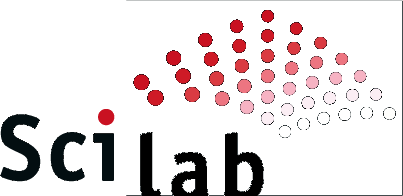
\includegraphics[height=.8cm]{png/logo_scilab}} 
\rotatebox{90}{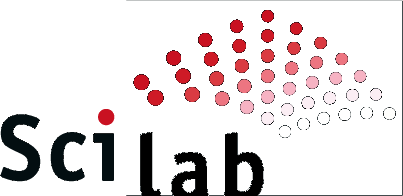
\includegraphics[height=.6cm]{png/logo_scilab}} 
        {\color{violetf}\vrule width 3pt}%
        \hspace{0pt}%must no space.
        \fboxsep=\FrameSep\colorbox{violetc}%
    }%
    \MakeFramed{\hsize #1 \advance\hsize-\width\FrameRestore}%
}%
{\endMakeFramed}%

\newenvironment{pseudo}[1][\hsize]%
{%
    \def\FrameCommand%
    {%
\rotatebox{90}{\textit{\textsf{Pseudo Code}}} 
        {\color{violetf}\vrule width 3pt}%
        \hspace{0pt}%must no space.
        \fboxsep=\FrameSep\colorbox{violetc}%
    }%
    \MakeFramed{\hsize #1 \advance\hsize-\width\FrameRestore}%
}%
{\endMakeFramed}%

\newenvironment{py}[1][\hsize]%
{%
    \def\FrameCommand%
    {%
%\rotatebox{90}{\textit{\textsf{Python}}} 
\rotatebox{90}{
\includegraphics[height=.6cm]{png/logo_python}} 
        {\color{violetf}\vrule width 3pt}%
        \hspace{0pt}%must no space.
        \fboxsep=\FrameSep\colorbox{violetc}%
    }%
    \MakeFramed{\hsize #1 \advance\hsize-\width\FrameRestore}%
}%
{\endMakeFramed}%


\newenvironment{term}[1][\hsize]%
{%
    \def\FrameCommand%
    {%
\rotatebox{90}{\textit{\textsf{Terminal}}} 
        {\color{violetf}\vrule width 3pt}%
        \hspace{0pt}%must no space.
        \fboxsep=\FrameSep\colorbox{violetc}%
    }%
    \MakeFramed{\hsize #1 \advance\hsize-\width\FrameRestore}%
}%
{\endMakeFramed}%



\newenvironment{comp}[1][\hsize]%
{%
    \def\FrameCommand
    {%
\rotatebox{90}{\textit{\textsf{Compétences}}} 
        {\color{bleuf}\vrule width 3pt}%
        \hspace{0pt}%must no space.
        \fboxsep=\FrameSep\colorbox{bleuc}%
    }%
    \MakeFramed{\hsize#1\advance\hsize-\width\FrameRestore}%
}%
{\endMakeFramed}%

\newenvironment{rem}[1][\hsize]%
{%
    \def\FrameCommand
    {%
\rotatebox{90}{\textit{\textsf{Remarque}}} 
        {\color{bleuf}\vrule width 3pt}%
        \hspace{0pt}%must no space.
        \fboxsep=\FrameSep\colorbox{bleuc}%
    }%
    \MakeFramed{\hsize#1\advance\hsize-\width\FrameRestore}%
}%
{\endMakeFramed}%


\newenvironment{savoir}[1][\hsize]%
{%
    \def\FrameCommand
    {%
\rotatebox{90}{\textit{\textsf{Savoir}}} 
        {\color{bleuf}\vrule width 3pt}%
        \hspace{0pt}%must no space.
        \fboxsep=\FrameSep\colorbox{bleuc}%
    }%
    \MakeFramed{\hsize#1\advance\hsize-\width\FrameRestore}%
}%
{\endMakeFramed}%

\newenvironment{Objectif}[1][\hsize]%
{%
    \def\FrameCommand
    {%
\rotatebox{90}{\textit{\textsf{Objectif}}} 
        {\color{bleuf}\vrule width 3pt}%
        \hspace{0pt}%must no space.
        \fboxsep=\FrameSep\colorbox{bleuc}%
    }%
    \MakeFramed{\hsize#1\advance\hsize-\width\FrameRestore}%
}%
{\endMakeFramed}%

\newenvironment{prob}[1][\hsize]%
{%
    \def\FrameCommand%
    {%
\rotatebox{90}{\textit{\textsf{ Problématique}}} 
        {\color{rougef}\vrule width 3pt}%
        \hspace{0pt}%must no space.
        \fboxsep=\FrameSep\colorbox{rougec}%
    }%
    \MakeFramed{\hsize#1\advance\hsize-\width\FrameRestore}%
}%
{\endMakeFramed}%

\newenvironment{obj}[1][\hsize]%
{%
    \def\FrameCommand%
    {%
\rotatebox{90}{\textit{\textsf{Objectifs}}} 
        {\color{rougef}\vrule width 3pt}%
        \hspace{0pt}%must no space.
        \fboxsep=\FrameSep\colorbox{rougec}%
    }%
    \MakeFramed{\hsize#1\advance\hsize-\width\FrameRestore}%
}%
{\endMakeFramed}%

\newenvironment{defi}[1][\hsize]%
{%
    \def\FrameCommand%
    {%
\rotatebox{90}{\textit{\textsf{Définition\\}}} 
        {\color{bleuf}\vrule width 3pt}%
        \hspace{0pt}%must no space.
        \fboxsep=\FrameSep\colorbox{bleuc}%
    }%
    \MakeFramed{\hsize#1\advance\hsize-\width\FrameRestore}%
}%
{\endMakeFramed}%


\newenvironment{demo}[1][\hsize]%
{%
    \def\FrameCommand%
    {%
\rotatebox{90}{\textit{\textsf{Démonstration\\}}} 
        {\color{bleuf}\vrule width 3pt}%
        \hspace{0pt}%must no space.
        \fboxsep=\FrameSep\colorbox{bleuc}%
    }%
    \MakeFramed{\hsize#1\advance\hsize-\width\FrameRestore}%
}%
{\endMakeFramed}%


\newenvironment{hypo}[1][\hsize]%
{%
    \def\FrameCommand%
    {%
\rotatebox{90}{\textit{\textsf{Hypothèse\\}}} 
        {\color{bleuf}\vrule width 3pt}%
        \hspace{0pt}%must no space.
        \fboxsep=\FrameSep\colorbox{bleuc}%
    }%
    \MakeFramed{\hsize#1\advance\hsize-\width\FrameRestore}%
}%
{\endMakeFramed}%


\newenvironment{prop}[1][\hsize]%
{%
    \def\FrameCommand%
    {%
\rotatebox{90}{\textit{\textsf{Propriété\\}}} 
        {\color{bleuf}\vrule width 3pt}%
        \hspace{0pt}%must no space.
        \fboxsep=\FrameSep\colorbox{bleuc}%
    }%
    \MakeFramed{\hsize#1\advance\hsize-\width\FrameRestore}%
}%
{\endMakeFramed}%

\newenvironment{props}[1][\hsize]%
{%
    \def\FrameCommand%
    {%
\rotatebox{90}{\textit{\textsf{Propriétés\\}}} 
        {\color{bleuf}\vrule width 3pt}%
        \hspace{0pt}%must no space.
        \fboxsep=\FrameSep\colorbox{bleuc}%
    }%
    \MakeFramed{\hsize#1\advance\hsize-\width\FrameRestore}%
}%
{\endMakeFramed}%

\newenvironment{exemple}[1][\hsize]%
{%
    \def\FrameCommand%
    {%
\rotatebox{90}{\textit{\textsf{Exemple\\}}} 
        {\color{vertf}\vrule width 3pt}%
        \hspace{0pt}%must no space.
        \fboxsep=\FrameSep\colorbox{vertc}%
    }%
    \MakeFramed{\hsize#1\advance\hsize-\width\FrameRestore}%
}%
{\endMakeFramed}%

\newenvironment{exercice}[1][\hsize]%
{%
    \def\FrameCommand%
    {%
\rotatebox{90}{\textit{\textsf{Exercice\\}}} 
        {\color{vertf}\vrule width 3pt}%
        \hspace{0pt}%must no space.
        \fboxsep=\FrameSep\colorbox{vertc}%
    }%
    \MakeFramed{\hsize#1\advance\hsize-\width\FrameRestore}%
}%
{\endMakeFramed}%

\newenvironment{Support}[1][\hsize]%
{%
    \def\FrameCommand%
    {%
\rotatebox{90}{\textit{\textsf{Support de cours\\}}} 
        {\color{vertf}\vrule width 3pt}%
        \hspace{0pt}%must no space.
        \fboxsep=\FrameSep\colorbox{jaunec}%
    }%
    \MakeFramed{\hsize#1\advance\hsize-\width\FrameRestore}%
}%
{\endMakeFramed}%

\newenvironment{resultat}[1][\hsize]%
{%
    \def\FrameCommand%
    {%
\rotatebox{90}{\textit{\textsf{Résultat\\}}} 
        {\color{rougef}\vrule width 3pt}%
        \hspace{0pt}%must no space.
        \fboxsep=\FrameSep\colorbox{rougec}%
    }%
    \MakeFramed{\hsize#1\advance\hsize-\width\FrameRestore}%
}%
{\endMakeFramed}%

\newenvironment{methode}[1][\hsize]%
{%
    \def\FrameCommand%
    {%
\rotatebox{90}{\textit{\textsf{Méthode\\}}} 
        {\color{rougef}\vrule width 3pt}%
        \hspace{0pt}%must no space.
        \fboxsep=\FrameSep\colorbox{rougec}%
    }%
    \MakeFramed{\hsize#1\advance\hsize-\width\FrameRestore}%
}%
{\endMakeFramed}%

\newenvironment{theo}[1][\hsize]%
{%
    \def\FrameCommand%
    {%
\rotatebox{90}{\textit{\textsf{Théorème\\}}} 
        {\color{rougef}\vrule width 3pt}%
        \hspace{0pt}%must no space.
        \fboxsep=\FrameSep\colorbox{rougec}%
    }%
    \MakeFramed{\hsize#1\advance\hsize-\width\FrameRestore}%
}%
{\endMakeFramed}%

\newenvironment{warn}[1][\hsize]%
{%
    \def\FrameCommand%
    {%
\rotatebox{90}{\textit{\textsf{Attention\\}}} 
        {\color{rougef}\vrule width 3pt}%
        \hspace{0pt}%must no space.
        \fboxsep=\FrameSep\colorbox{rougec}%
    }%
    \MakeFramed{\hsize#1\advance\hsize-\width\FrameRestore}%
}%
{\endMakeFramed}%

%Si le boolen xp est vrai : compilation pour xabi
%Sinon compilation Damien
\newboolean{xp}
\setboolean{xp}{true}

\newboolean{prof}
\setboolean{prof}{true}

\usepackage[%
    pdftitle={CI 06 : Stat - Ch 02 : PFS},
    pdfauthor={Xavier Pessoles},
    colorlinks=true,
    linkcolor=blue,
    citecolor=magenta]{hyperref}


\def\discipline{Sciences Industrielles de l'Ingénieur}
\def\xxtitre{\ifthenelse{\boolean{xp}}{
CI 6 : Étude du comportement statique des systèmes}{}}

\def\xxsoustitre{\ifthenelse{\boolean{xp}}{
Chapitre 2 -- Principe Fondamental de la Statique}{
Partie  -- }}

\def\xxauteur{\ifthenelse{\boolean{xp}}{
Xavier \textsc{Pessoles}}{}}

\def\xxpied{\ifthenelse{\boolean{xp}}{
CI 6 : Statique\\
Ch. 2 : PFS -- Cours}{
\xxtitre}}

\def\xxcathegorie{\ifthenelse{\boolean{xp}}{
2013 -- 2014 \\
Xavier \textsc{Pessoles}}{}}





%---------------------------------------------------------------------------


\begin{document}

\ifthenelse{\boolean{xp}}{
\sloppy
\hyphenpenalty 10000


%------------- En tetes et Pieds de Pages ------------

\pagestyle{fancy}
\renewcommand{\headrulewidth}{0pt}
\fancyhead{}
\fancyhead[L]{%
\noindent\begin{minipage}[c]{2.6cm}%

\includegraphics[width=2cm]{png/logo_ptsi.png}%
\end{minipage}}


\fancyhead[C]{\rule{12cm}{.5pt}}


\fancyhead[R]{%
\noindent\begin{minipage}[c]{3cm}
\begin{flushright}
\footnotesize{\textit{\textsf{\discipline}}}%
\end{flushright}
\end{minipage}
}



\fancyhead[C]{\rule{12cm}{.5pt}}

\renewcommand{\footrulewidth}{0.2pt}

\fancyfoot[C]{\footnotesize{\bfseries \thepage}}
\fancyfoot[L]{%
\begin{minipage}[c]{.4\linewidth}
\noindent\footnotesize{{\xxauteur}}
\end{minipage}
}

\fancyfoot[R]{\footnotesize{\xxpied}}

\begin{center}
 \iftd
 \Large\textsc{\xxtitre}
 \else
 \huge\textsc{\xxtitre}
 \fi
\end{center}

\begin{center}
 \iftd
 \large\textsc{\xxsoustitre}
 \else
 \LARGE\textsc{\xxsoustitre}
 \fi
\end{center}

\vspace{.5cm}
}{\ifthenelse{\boolean{xp}}{
\usepackage[%
    pdftitle={OS et Environnement de développement},
    pdfauthor={Xavier Pessoles},
    colorlinks=true,
    linkcolor=blue,
    citecolor=magenta]{hyperref}}{
\usepackage[%
    pdftitle={OS et Environnement de développement},
    pdfauthor={Damien Iceta},
    colorlinks=true,
    linkcolor=blue,
    citecolor=magenta]{hyperref}}

\usepackage{pifont}
\usepackage{lastpage}

% \makeatletter \let\ps@plain\ps@empty \makeatother
%% DEBUT DU DOCUMENT
%% =================
\sloppy
\hyphenpenalty 10000

\newcommand{\Pointilles}[1][3]{%
\multido{}{#1}{\makebox[\linewidth]{\dotfill}\\[\parskip]
}}


\colorlet{shadecolor}{orange!15}

\newtheorem{theorem}{Theorem}


\begin{document}


\newboolean{prof}
\setboolean{prof}{true}
%------------- En tetes et Pieds de Pages ------------


\pagestyle{fancy}
%\renewcommand{\headrulewidth}{0}
\renewcommand{\headrulewidth}{0.2pt} %pour mettre le trait en haut

\fancyhead{}
\fancyhead[L]{
\footnotesize{{{\xxtitre}}}%
%\noindent\noindent\begin{minipage}[c]{2.6cm}
%\includegraphics[width=2.5cm]{png/logo.png}%
%\end{minipage}
}

%\fancyhead[C]{\rule{12cm}{.5pt}}  %pour mettre le petit trait en haut


\fancyhead[R]{%
\noindent\begin{minipage}[c]{3cm}
\begin{flushright}
\footnotesize{{{\xxcathegorie}}}%
\end{flushright}
\end{minipage}
}

\renewcommand{\footrulewidth}{0.2pt}

\fancyfoot[C]{\footnotesize{}}
\fancyfoot[L]{%
\begin{minipage}[l]{.2\linewidth}
\noindent\footnotesize{{\xxauteur}}
\end{minipage}
\begin{minipage}[c]{.15\linewidth}
%
\includegraphics[width=2cm]{png/logoCC.png}
\end{minipage}}

\ifthenelse{\boolean{prof}}{%
\fancyfoot[R]{\footnotesize{Page \thepage\   sur  \pageref{LastPage}}}}

\begin{center}
 \huge\textsc{\xxtitre}
\end{center}

\begin{center}
 \LARGE\textsc{\xxsoustitre}
\end{center}

\vspace{.5cm}}





\begin{center}
\begin{tabular}{cc}
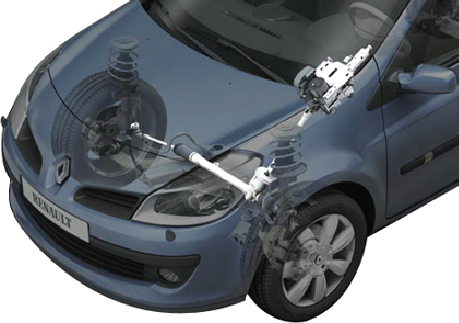
\includegraphics[height=3cm]{images/dae_renault} &
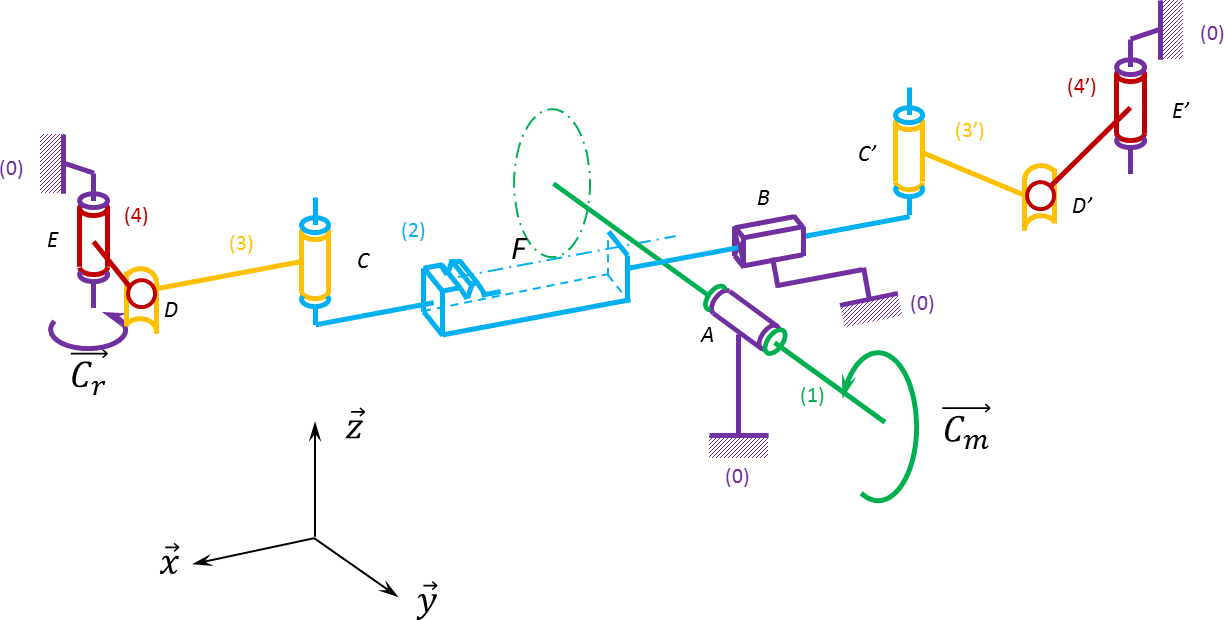
\includegraphics[height=5cm]{images/schema} \\
\textit{Direction assistée électrique de Clio \cite{clio}} & \textit{Modélisation cinématique de la DAE de Twingo}\\
\end{tabular}
\end{center}

\vspace{.2cm}

Sur un véhicule automobile, la direction assistée permet d'aider le conducteur à diriger le véhicule en fonction de sa vitesse. En effet, à basse vitesse, l'adhérence entre les pneus et le sol rend difficile les manœuvres. Sur le système de direction assistée présenté ci-dessus, un moteur électrique lié à la colonne de direction par l'intermédiaire d'un réducteur roue-vis sans fin permet de restituer un couple d'assistance. 

On cherche à dimensionner le moteur électrique pour qu'il fournisse un couple suffisant dans le but d'aider le conducteur. 

\begin{prob}
\textsc{Problématique :}
\begin{itemize}
\item Comment calculer les efforts dans les liaisons d'un système mécanique ?
\item Comment déterminer le couple maximal à fournir par le moteur électrique d'assistance ?
\end{itemize}
\end{prob}

\begin{savoir}
\textsc{Savoirs :}
\begin{itemize}
\item Mod -- C15 : Modélisation des actions mécaniques : 
\begin{itemize}
\item Mod -- C15.4 : Principe fondamental de la statique
\item Mod -- C15 -- S5  : Appliquer le PFS à un solide ou à un système de solides. 
\end{itemize}
\item Rés -- C2 : Actions mécaniques dans les liaisons, équations de mouvement
\begin{itemize}
\item Rés -- C2.1 : Théorème des actions réciproques
\item Rés -- C2.S1 : Choisir un modèle et une méthode de résolution (choix des isolements et théorèmes appliquées). 
\item Rés -- C2.S2 : Déterminer les actions mécaniques désirées.
\end{itemize}
\end{itemize}
\end{savoir}

\setlength{\parskip}{0ex plus 0.2ex minus 0ex}
 \renewcommand{\contentsname}{}
 \renewcommand{\baselinestretch}{1}

\tableofcontents

 \renewcommand{\baselinestretch}{1.2}
\setlength{\parskip}{2ex plus 0.5ex minus 0.2ex}

% \vspace{1cm}
\textit{Ce document est en évolution permanente. Merci de signaler toutes
erreurs ou coquilles.}

\section{Principe fondamental de la statique -- PFS}
\begin{theo}
\textbf{Principe fondamental de la statique -- PFS}

On note $S$ un système matériel à l'équilibre et $\overline{S}$ le milieu extérieur à ce système.

$S$ est à l'équilibre par rapport à un repère galiléen $\mathcal{R}$ si $\forall M \in S$, $\left[\dfrac{d\vect{OM}}{dt}\right]_{\mathcal{R}}=\vect{0}$.

Si $S$ est à l'équilibre, alors : 
$$
\left\{ \mathcal{T} \left( \overline{S} \rightarrow  S\right)\right\} =\{0\}
$$

$\left\{ \mathcal{T}\left( \overline{S} \rightarrow  S\right)\right\}$ désigne la somme des actions mécaniques agissant sur $S$.
\end{theo}


\begin{exemple}
\begin{minipage}[c]{.65\linewidth}
On isole le solide $3$. Si on néglige la pesanteur, le solide est soumis à l'action de la liaison linéaire annulaire et de l'action de la liaison pivot. 
\end{minipage}\hfill
\begin{minipage}[c]{.3\linewidth}
\begin{center}
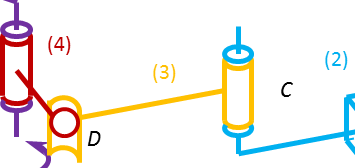
\includegraphics[width=.8\textwidth]{images/3}
\end{center}
\end{minipage}
Le PFS appliqué au solide $3$ au point $C$ s'écrit donc ainsi : 
$$
\torseurstat{T}{4}{3} + \torseurstat{T}{2}{3} = \{0\}
$$
En écrivant les torseurs au point $C$  ($\vect{CD}=-\lambda\vect{x}$):
$$
\torseurstat{T}{4}{3}
=\torseurcol{X_{43}}{Y_{43}}{0}{0}{0}{0}{D,\mathcal{R}}
=\torseurcol{X_{43}}{Y_{43}}{0}{0}{0}{-\lambda Y_{43}}{C,\mathcal{R}}
\quad
\torseurstat{T}{2}{3}
=\torseurcol{X_{23}}{Y_{23}}{Z_{23}}{L_{23}}{M_{23}}{0}{C,\mathcal{R}}
$$
On a donc : 
$$
\torseurcol{X_{43}}{Y_{43}}{0}{0}{0}{-\lambda Y_{43}}{C,\mathcal{R}}
+ \torseurcol{X_{23}}{Y_{23}}{Z_{23}}{L_{23}}{M_{23}}{0}{C,\mathcal{R}}
= \torseurcol{0}{0}{0}{0}{0}{0}{C,\mathcal{R}}
$$
\end{exemple}


\begin{theo}
\textbf{Équations vectorielles du PFS}

De l'écriture sous forme de torseurs découle deux théorèmes.

Théorème de la résultante statique :
$$
\vectf{\overline{S}}{S}=\vect{0}
$$

Théorème du moment statique au point M :
$$
\vectm{M}{\overline{S}}{S}=\vect{0}
$$

Deux ces 2 équations vectorielles en 3 dimension, on peut donc déduire un système à 6 équations.
\end{theo}

\begin{exemple}
Le théorème de la résultante statique appliqué au solide $3$ s'écrit :
$$
\vectf{4}{3}+\vectf{2}{3}=\vect{0}
$$

Le théorème du moment statique appliqué au solide $3$ au point $C$ s'écrit :
$$
\vectm{C}{4}{3}+\vectm{C}{2}{3}=\vect{0}
$$

\end{exemple}


\begin{theo}
\textbf{Théorème des actions réciproques}

Soient $S_1$ et $S_2$ deux systèmes mécaniques en équilibre. On a donc : 
$$
\torseurstat{T}{S_2}{S_1}=-\torseurstat{T}{S_1}{S_2}
$$
\end{theo}

\begin{exemple}
$$
\torseurstat{T}{2}{3}
=-\torseurstat{T}{3}{2} \Longleftrightarrow
\torseurl{\vectf{2}{3}}{\vectm{C}{2}{3}}{C,\mathcal{R}}
=
\torseurl{-\vectf{3}{2}}{-\vectm{C}{3}{2}}{C,\mathcal{R}}
$$
$$
\torseurcol{X_{23}}{Y_{23}}{Z_{23}}{L_{23}}{M_{23}}{0}{C,\mathcal{R}} =
\torseurcol{-X_{32}}{-Y_{32}}{-Z_{32}}{-L_{32}}{-M_{32}}{0}{C,\mathcal{R}}
$$
\end{exemple}

\section{Résolution d'un problème en statique}

Lors de la résolution d'un problème en statique, les difficultés sont entre autres : 
\begin{itemize}
\item modéliser le problème;
\item définir le système mécanique auquel on désire appliquer PFS;
\item faire le bilan exhaustif des actions mécaniques agissant sur le système;
\item en fonction du problème, choisir au mieux le théorème à utiliser pour éviter trop de calculs.
\end{itemize}

Dans la suite, on cherche d'une part à calculer le couple moteur afin de dimensionner le moteur d'assistance. D'autre part, on cherche à déterminer les efforts dans les liaisons dans le but de pouvoir les dimensionner.

Le couple résistant $\vect{C_r}$ est connu.

\subsection{Modélisation du système}
Deux outils permettent de modéliser un système en vu de la résolution d'un problème de statique : le schéma d'architecture et le graphe de structure. Ils permettent de traduire par des liaisons cinématiques chacun des contacts entre les différentes classes d'équivalence cinématiques d'un système.

\begin{center}
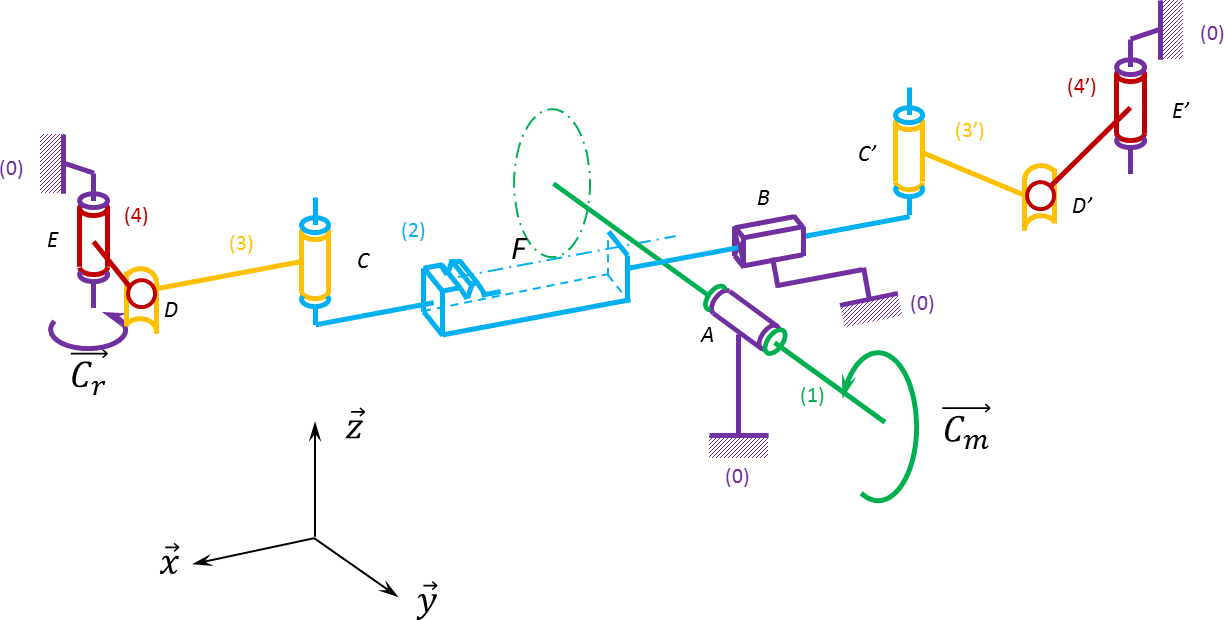
\includegraphics[width=\textwidth]{images/schema}
\textit{Schéma d'architecture}
\end{center}

\begin{center}
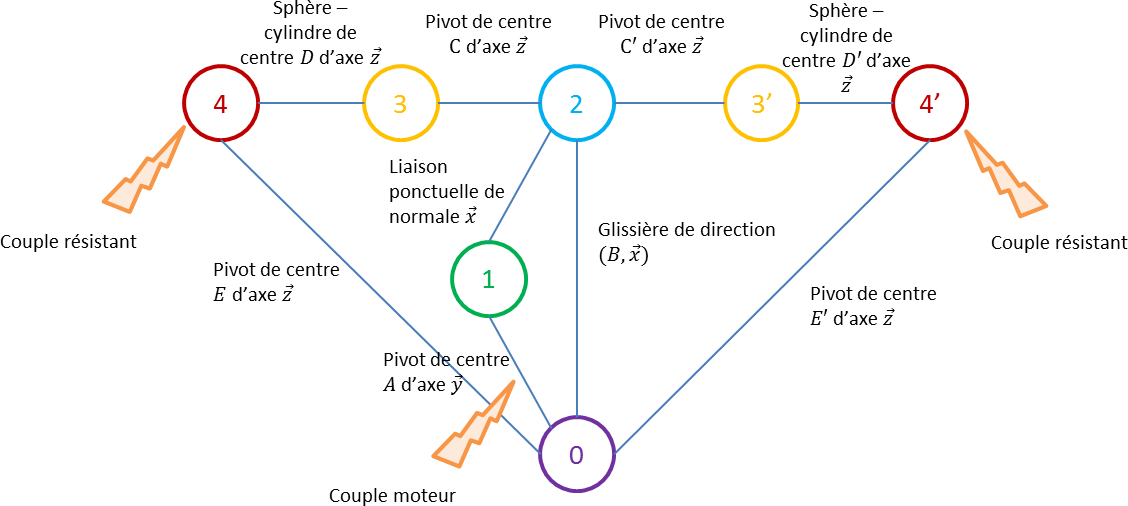
\includegraphics[width=\textwidth]{images/graphe}
\textit{Graphe de structure}
\end{center}

\subsection{Recherche des inconnues dans les liaisons}
\begin{obj}
L'objectif est ici de déterminer les composantes du torseur statique.
\end{obj}
\subsubsection{Bilan des actions mécaniques extérieures}
\begin{rem}
Le but est ici de donner l'ensemble des torseurs d'actions mécaniques exerçant sur le système. 
\end{rem}

\paragraph*{Actions à distance}
La seule action à distance est ici la pesanteur. 

\setlength{\columnseprule}{0.4pt}

%\columnseprule{.4}

\begin{multicols}{2}


Action de la pesanteur agissant sur la pièce 1 en son centre d'inertie $G_1$ :
$$
\torseurstat{T}{\text{pes}}{1} =
\torseurl{%
\vectf{\text{pes}}{1}=-M_1g\vect{z}}{%
\vectm{G_1}{\text{pes}}{1}=\vect{0}}{G_1,\mathcal{R}}
$$

Action de la pesanteur agissant sur la pièce 2 en son centre d'inertie $G_2$ :
$$
\torseurstat{T}{\text{pes}}{2} =
\torseurl{%
\vectf{\text{pes}}{2}=-M_2g\vect{z}}{%
\vectm{G_2}{\text{pes}}{2}=\vect{0}}{G_2,\mathcal{R}}
$$

Action de la pesanteur agissant sur la pièce 3 en son centre d'inertie $G_3$ :
$$
\torseurstat{T}{\text{pes}}{3} =
\torseurl{%
\vectf{\text{pes}}{3}=-M_3g\vect{z}}{%
\vectm{G_3}{\text{pes}}{3}=\vect{0}}{G_3,\mathcal{R}}
$$

Action de la pesanteur agissant sur la pièce 4 en son centre d'inertie $G_4$ :
$$
\torseurstat{T}{\text{pes}}{4} =
\torseurl{%
\vectf{\text{pes}}{4}=-M_4g\vect{z}}{%
\vectm{G_4}{\text{pes}}{4}=\vect{0}}{G_4,\mathcal{R}}
$$


Action de la pesanteur agissant sur la pièce 3' en son centre d'inertie $G_3'$ :
$$
\torseurstat{T}{\text{pes}}{3'} =
\torseurl{%
\vectf{\text{pes}}{3'}=-M_3'g\vect{z}}{%
\vectm{G_3'}{\text{pes}}{3'}=\vect{0}}{G_3',\mathcal{R}}
$$

Action de la pesanteur agissant sur la pièce 4' en son centre d'inertie $G_4'$ :
$$
\torseurstat{T}{\text{pes}}{4'} =
\torseurl{%
\vectf{\text{pes}}{4'}=-M_4'g\vect{z}}{%
\vectm{G_4'}{\text{pes}}{4'}=\vect{0}}{G_4',\mathcal{R}}
$$

\end{multicols}

\newpage 

\paragraph*{Action dans les liaisons cinématiques}

\begin{multicols}{2}
Action de la liaison pivot d'axe $\vect{y}$ de 0 sur 1 en $A$ :
$$
\torseurstat{T}{0}{1} =
\torseurcol{X_{01}}{Y_{01}}{Z_{01}}{L_{01}}{0}{N_{01}}{A,\mathcal{R}}
$$

Action de la liaison glissière d'axe $\vect{x}$ de 0 sur 2 en $B$ :
$$
\torseurstat{T}{0}{2} =
\torseurcol{0}{Y_{02}}{Z_{02}}{L_{02}}{M_{02}}{N_{02}}{B,\mathcal{R}}
$$

Action de la liaison ponctuelle de normale $\vect{x}$ de 1 sur 2 en $F$ (pignon -- crémaillère):
$$
\torseurstat{T}{1}{2} =
\torseurcol{X_{12}}{0}{0}{0}{0}{0}{F,\mathcal{R}}
$$


Action de la liaison pivot d'axe $\vect{z}$ de 2 sur 3 en $C$ :
$$
\torseurstat{T}{2}{3} =
\torseurcol{X_{23}}{Y_{23}}{Z_{23}}{L_{23}}{M_{23}}{0}{C,\mathcal{R}}
$$

Action de la liaison sphère--cylindre d'axe $\vect{z}$ de 3 sur 4 en $D$ :
$$
\torseurstat{T}{3}{4} =
\torseurcol{X_{34}}{Y_{34}}{0}{0}{0}{0}{D,\mathcal{R}}
$$

Action de la liaison pivot d'axe $\vect{z}$ de 0 sur 4 en $E$ :
$$
\torseurstat{T}{0}{4} =
\torseurcol{X_{04}}{Y_{04}}{Z_{04}}{L_{04}}{M_{04}}{0}{E,\mathcal{R}}
$$



Action de la liaison pivot d'axe $\vect{z}$ de 2 sur 3' en $C'$ :
$$
\torseurstat{T}{2}{3'} =
\torseurcol{X_{23'}}{Y_{23'}}{Z_{23'}}{L_{23'}}{M_{23'}}{0}{C',\mathcal{R}}
$$

Action de la liaison sphère--cylindre d'axe $\vect{z}$ de 3' sur 4' en $D'$ :
$$
\torseurstat{T}{3'}{4'} =
\torseurcol{X_{3'4'}}{Y_{3'4'}}{0}{0}{0}{0}{D',\mathcal{R}}
$$



Action de la liaison pivot d'axe $\vect{z}$ de 0 sur 4 en $E'$ :
$$
\torseurstat{T}{0'}{4'} =
\torseurcol{X_{0'4'}}{Y_{0'4'}}{Z_{0'4'}}{L_{0'4'}}{M_{0'4'}}{0}{E',\mathcal{R}}
$$

\end{multicols}

\paragraph*{Actions de contact}
\begin{multicols}{3}
Action du couple moteur agissant sur la pièce 1 en $A$ :
$$
\torseurstat{T}{\text{moteur}}{1}=
\torseurcol{0}{0}{0}{0}{C_m}{0}{A,\mathcal{R}}
$$


Action du couple résistant agissant sur la pièce 4 en $E$ :
$$
\torseurstat{T}{\text{res}}{4}=
\torseurcol{0}{0}{0}{0}{0}{C_r}{E,\mathcal{R}}
$$

Action du couple résistant agissant sur la pièce 4' en $E'$ :
$$
\torseurstat{T}{\text{res}}{4'}=
\torseurcol{0}{0}{0}{0}{0}{C_r'}{E',\mathcal{R}}
$$
\end{multicols}

\paragraph*{Bilan des actions mécaniques}
Au bilan, le poids de chaque pièce est connu ainsi que les couples de frottements dans les liaisons pivots entre 0 et 4 et entre 0 et 4'. 

Il y a 35 inconnues de liaisons et une action mécanique inconnue : le couple moteur. 

\textbf{Il y a donc 36 inconnues dans ce système.}

\subsubsection{Calcul des actions mécaniques dans la pièce 4}

\textbf{Isolons le solide 4}. 

4 est soumis à la pesanteur, au couple résistant et aux actions de liaisons entre 4 et 0 et entre 3 et 4. Ces torseurs ont été écrits précédemment.

\begin{center}
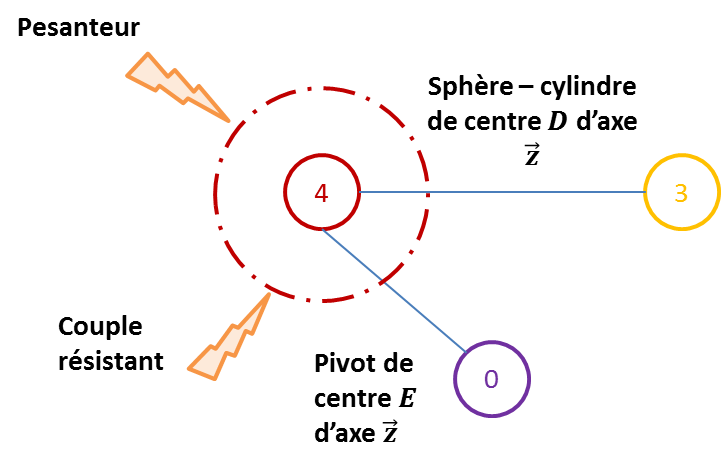
\includegraphics[width=.6\textwidth]{images/4}
\end{center}

\begin{rem}
En isolant le solide 4, on est en présence de 7 inconnues (5 inconnues de liaisons dans la liaison pivot 2 inconnues dans la liaison linéaire annulaire). Le PFS va permettre d'écrire 6 équations. Il n'est donc pas \textit{a priori} possible de déterminer toutes les inconnues.
\end{rem}

\textbf{Appliquons le PFS au solide 4 au point $E$ :}
$$
\torseurstat{T}{\text{res}}{4} 
+ \torseurstat{T}{\text{pes}}{4}
+ \torseurstat{T}{0}{4}
+ \torseurstat{T}{3}{4}
=\left\{ 0\right\}
$$

Pour appliquer le PFS, il faut donc écrire chacun des torseurs en un point. Nous avons choisi le point $E$. Le point $E$ est choisi car deux torseurs y sont déjà connus.

On note : $\vect{EG_4} = x_{G_4}\vect{x}+y_{G_4}\vect{y}+z_{G_4}\vect{z}$ et 
$\vect{ED} = x_D\vect{x}+y_D\vect{y}$.


Exprimons le torseur de pesanteur au point $E$ :
$$
\torseurstat{T}{\text{pes}}{4} =
\torseurl{%
\vectf{\text{pes}}{4}=-M_4g\vect{z}}{%
\vectm{E}{\text{pes}}{4}=\underbrace{\vectm{G_4}{\text{pes}}{4}}_{\vect{0}}+\vect{EG_4}\wedge\vectf{\text{pes}}{4}=
\left( x_{G_4}\vect{x}+y_{G_4}\vect{y}+z_{G_4}\vect{z}\right) \wedge \left(-M_4g\vect{z}\right)
}{G_4,\mathcal{R}}
$$
$$
\vectm{E}{\text{pes}}{4}= M_4gx_{G_4}\vect{y}-M_4gy_{G_4}\vect{x}
$$

$$
\torseurstat{T}{\text{pes}}{4} =
\torseurl{%
\vectf{\text{pes}}{4}=-M_4g\vect{z}}{%
\vectm{E}{\text{pes}}{4}= M_4gx_{G_4}\vect{y}-M_4gy_{G_4}\vect{x}
}{E,\mathcal{R}}
=\torseurcol{0}{0}{-M_4g}{-y_{G_4}M_4g}{x_{G_4}M_4g}{0}{E,\mathcal{R}}
$$

Exprimons le torseur liaison entre 3 et 4 au point $E$ :
$$
\torseurstat{T}{3}{4} =
\torseurcol{X_{34}}{Y_{34}}{0}{0}{0}{0}{D,\mathcal{R}}
=\left\{
\overbrace{\left|
\begin{array}{c}
X_{34} \\ Y_{34} \\ 0
\end{array}
\right.}^{\vect{R}}
\quad\quad
\overbrace{\left|
\begin{array}{c}
0 \\ 0\\0
\end{array}
\right.}^{\vect{\mathcal{M}_D}}
+
\overbrace{\left|
\begin{array}{c}
x_D \\ y_D \\ 0
\end{array}
\right.}^{\vect{ED}}
\wedge
\overbrace{\left|
\begin{array}{c}
X_{34} \\ Y_{34} \\ 0
\end{array}
\right.}^{\vect{R}}
\right\}_{E,\mathcal{R}}
=
\torseurcol{X_{34}}{Y_{34}}{0}{0}{0}{x_DY_{34}-y_DX_{34}}{E,\mathcal{R}}
$$

Tous les torseurs sont appliqués au point $E$. On peut donc appliquer le PFS :
$$
\torseurcol{0}{0}{0}{0}{0}{C_r}{E,\mathcal{R}}+
\torseurcol{X_{34}}{Y_{34}}{0}{0}{0}{x_DY_{34}-y_DX_{34}}{E,\mathcal{R}}
+
\torseurcol{0}{0}{-M_4g}{-y_{G_4}M_4g}{x_{G_4}M_4g}{0}{E,\mathcal{R}}
+
\torseurcol{X_{04}}{Y_{04}}{Z_{04}}{L_{04}}{M_{04}}{0}{E,\mathcal{R}}
=
\torseurcol{0}{0}{0}{0}{0}{0}{D,\mathcal{R}}
$$

On peut donc écrire un système de 6 équations avec chacune des composantes de chacun des vecteurs :
$$
\left\{
\begin{array}{l}
{0}+{X_{34}}+{0}+{X_{04}}=0 \\
{0}+{Y_{34}}+{0}+{Y_{04}}=0 \\
{0}+{0}{-M_4g}+{Z_{04}}=0 \\
{0}+{0}{-y_{G_4}M_4g}+{L_{04}}=0 \\
{0}+{0}+{x_{G_4}M_4g}+{M_{04}}=0 \\
{C_r}+{x_DY_{34}-y_DX_{34}}+{0}+{0}=0 \\
\end{array}
\right.
\Longleftrightarrow
\left\{
\begin{array}{l}
{X_{34}}+{X_{04}}=0 \\
{Y_{34}}+{Y_{04}}=0 \\
{-M_4g}+{Z_{04}}=0 \\
{-y_{G_4}M_4g}+{L_{04}}=0 \\
{x_{G_4}M_4g}+{M_{04}}=0 \\
{C_r}+{x_DY_{34}-y_DX_{34}}=0 \\
\end{array}
\right.
\Longleftrightarrow
\left\{
\begin{array}{l}
{X_{34}}+{X_{04}}=0 \\
{Y_{34}}+{Y_{04}}=0 \\
{Z_{04}}=M_4g \\
{L_{04}}={y_{G_4}M_4g}\\
{M_{04}}=- {x_{G_4}M_4g}\\
{C_r}+{x_DY_{34}-y_DX_{34}}=0 \\
\end{array}
\right.
$$

Comme prévu, le système d'équations ne permet pas d'isoler les inconnues.

\textbf{Pour simplifier les calculs, nous négligerons l'effet du poids par la suite.}

\vspace{.5cm}
\begin{minipage}[c]{.45\linewidth}
En isolant le solide 4, le PFS au point $E$ devient donc : 
$$
\left\{
\begin{array}{l}
{X_{34}}+{X_{04}}=0 \\
{Y_{34}}+{Y_{04}}=0 \\
{Z_{04}}=0 \\
{L_{04}}=0\\
{M_{04}}=0\\
{C_r}+{x_DY_{34}-y_DX_{34}}=0 \\
\end{array}
\right.
$$

\end{minipage} \hfill
\begin{minipage}[c]{.45\linewidth}
Par symétrie, en isolant le solide 4', le PFS au point $E'$ s'écrit ainsi : 
$$
\left\{
\begin{array}{l}
{X_{3'4'}}+{X_{04'}}=0 \\
{Y_{3'4'}}+{Y_{04'}}=0 \\
{Z_{04'}}=0 \\
{L_{04'}}=0\\
{M_{04'}}=0\\
{C_r}+{x_D'Y_{3'4'}-y_D'X_{3'4'}}=0 \\
\end{array}
\right.
$$

\end{minipage}


\begin{rem}
A ce stade, restent à déterminer les 8 inconnues suivantes : $X_{34}$, $X_{04}$, $Y_{34}$, $Y_{04}$, $X_{3'4'}$, $X_{04'}$, $Y_{3'4'}$ et $Y_{04'}$.

6 équations n'ont pas encore été utilisées.

2 équations supplémentaires sont donc nécessaires pour calculer les inconnues. 

Il faudrait donc réaliser d'autres isolements et leur appliquer le PFS pour pouvoir déterminer les inconnues manquantes.
\end{rem}



\subsection{Recherche d'une relation entre le couple moteur et l'action dans la liaison pignon-crémaillère}

Dans certain cas il n'est pas indispensable d'appliquer le PFS dans sa totalité. L'application du théorème de la résultante statique ou du moment statique en un point peut suffire. En allant un peu plus loin, seule la projection d'un des théorèmes peut suffire.

Dans notre cas, commençons par \textbf{isoler le solide 1}.

$1$ est soumis au couple moteur, à la sphère -- plan en $I$, à la liaison pivot de centre $A$.

Nous souhaitons une relation entre $C_m$ et $X_{12}$. Par ailleurs, la liaison pivot ne transmet pas de couple autour de $\vect{y}$. On va donc appliquer le théorème du moment statique en A en projection autour de l'axe $\vect{y}$.

Commençons par déplacer le torseur $\torseurstat{T}{1}{2}$ (pignon -- crémaillère) au point $A$. On note $\vect{AF}=-L\vect{y}-R\vect{z}$.


$$
\vectm{A}{1}{2} = \vectm{F}{1}{2} + \vect{AF}\wedge\vectf{1}{2} 
= \left(-L\vect{y}-R\vect{z}\right) \wedge X_{12} \vect{x}
=LX_{12}\vect{z}-RX_{12}\vect{y}
$$

$$
\torseurstat{T}{1}{2} 
=\torseurcol{X_{12}}{0}{0}{0}{0}{0}{F,\mathcal{R}}
=\torseurcol{X_{12}}{0}{0}{0}{-RX_{12}}{LX_{12}}{A,\mathcal{R}}
\Longleftrightarrow
\torseurstat{T}{2}{1} 
=\torseurcol{-X_{12}}{0}{0}{0}{RX_{12}}{-LX_{12}}{A,\mathcal{R}}
$$

Par ailleurs, 
$$
\torseurstat{T}{\text{moteur}}{1}=
\torseurcol{0}{0}{0}{0}{C_m}{0}{A,\mathcal{R}}
 \quad \quad
\torseurstat{T}{0}{1} =
\torseurcol{X_{01}}{Y_{01}}{Z_{01}}{L_{01}}{0}{N_{01}}{A,\mathcal{R}}
$$


L'application du théorème du moment statique au point A sur l'axe $\vect{y}$ se traduit donc par l'équation suivante :
$$
R X_{12} + C_m = 0
$$




\subsection{Résolution finale du problème}
Le problème de choix du moteur d'assistance demande d'établir le lien entre :
\begin{itemize}
\item le couple de frottement entre la route et les pneus;
\item le couple moteur.
\end{itemize}

\subsubsection*{Ensemble soumis à 2 actions mécaniques}
\textbf{Isolons le solide $3$}

\textbf{Bilan des actions mécanique extérieures à 3}
$\vect{CD}=a\vect{x}$

$$
\torseurstat{T}{4}{3} 
= \torseurcol{X_{43}}{Y_{43}}{0}{0}{0}{0}{D,\mathcal{R}}
= \torseurcol{X_{43}}{Y_{43}}{0}{0}{0}{aY_{43}}{C,\mathcal{R}}
\quad
\torseurstat{T}{2}{3} 
= \torseurcol{X_{23}}{Y_{23}}{Z_{23}}{L_{23}}{M_{23}}{0}{C,\mathcal{R}}
$$

\textbf{Théorème du moment statique appliqué à 3 en $C$ en projection suivant $\vect{z}$ :}
$$
aY_{43}=0 \Longleftrightarrow Y_{43}=0
$$

Par analogie, le théorème du moment statique appliqué à 3' en $C'$ en projection suivant $\vect{z}$ 
$$
Y_{4'3'}=0
$$

\subsubsection*{Ensemble soumis à 4 actions mécaniques}
\textbf{Isolons l'ensemble $S=\{ 2+3+3'\}$}

\textbf{Bilan des actions mécanique extérieures au système}

Ce système est soumis aux actions des liaisons sphères cylindres en $D$ et $D'$, à la liaison ponctuelle en $F$ et la glissière en $B$. Déplaçons les torseurs au point $B$.

\begin{center}
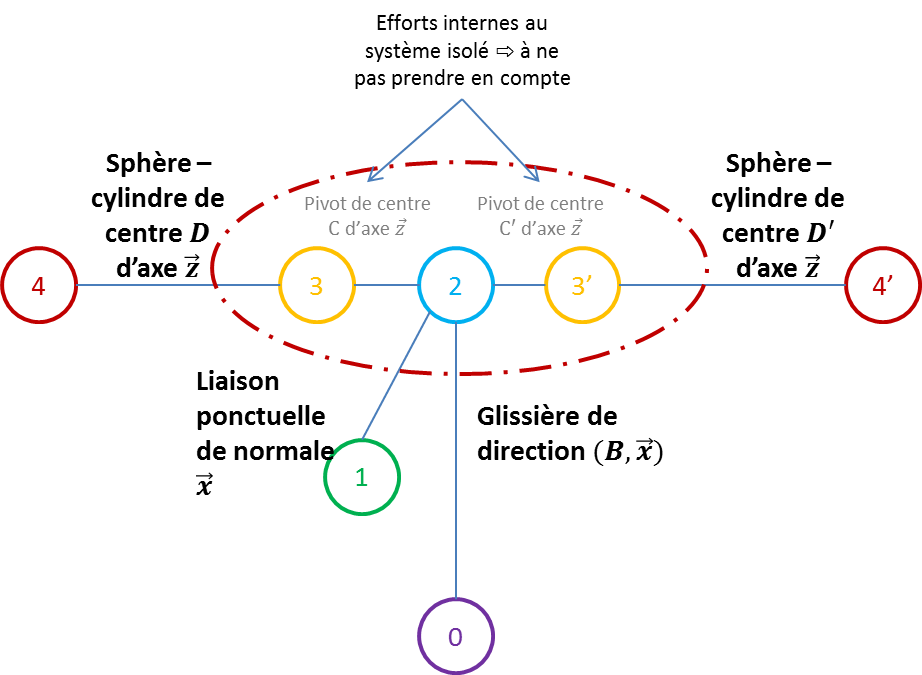
\includegraphics[width=.75\textwidth]{images/E}
\end{center}
$$
\torseurstat{T}{4}{3} 
= \torseurcol{X_{43}}{Y_{43}}{0}{0}{0}{0}{D,\mathcal{R}}
\;
\torseurstat{T}{4'}{3'} 
= \torseurcol{X_{4'3'}}{Y_{4'3'}}{0}{0}{0}{0}{D',\mathcal{R}}
$$
$$
\torseurstat{T}{1}{2} 
= \torseurcol{X_{12}}{0}{0}{0}{0}{0}{F,\mathcal{R}}
\;
\torseurstat{T}{0}{2} =
\torseurcol{0}{Y_{02}}{Z_{02}}{L_{02}}{M_{02}}{N_{02}}{B,\mathcal{R}}
$$

En appliquant le théorème de la résultante statique : à l'ensemble $S$ en projection sur l'axe $\vect{x}$ :
$$
X_{43}+X_{4'3'}+X_{12}=0
$$



\subsubsection*{Bilan}
A l'aide des équations déterminées précédemment on a : 

$$
\left\{
\begin{array}{l}
{X_{34}}+{X_{04}}=0 \\
{Y_{34}}+{Y_{04}}=0 \\
{Z_{04}}=0 \\
{L_{04}}=0\\
{M_{04}}=0\\
{C_r}+{x_DY_{34}-y_DX_{34}}=0 \\
\end{array}
\right.
\quad \quad
\left\{
\begin{array}{l}
{X_{3'4'}}+{X_{04'}}=0 \\
{Y_{3'4'}}+{Y_{04'}}=0 \\
{Z_{04'}}=0 \\
{L_{04'}}=0\\
{M_{04'}}=0\\
{C_r'}+{x_D'Y_{3'4'}-y_D'X_{3'4'}}=0 \\
\end{array}
\right.
\quad 
\left\{
\begin{array}{l}
R X_{12} + C_m = 0\\
X_{43}+X_{4'3'}+X_{12}=0\\
Y_{4'3'}=0\\
Y_{4'3'}=0
\end{array}
\right.
$$


$$
\Longrightarrow
\left\{
\begin{array}{l}
{X_{34}}+{X_{04}}=0 \\
{C_r}-y_DX_{34}=0 \\
{X_{3'4'}}+{X_{04'}}=0 \\
{C_r'}-y_D'X_{3'4'}=0 \\
R X_{12} + C_m = 0\\
X_{43}+X_{4'3'}+X_{12}=0\\
\end{array}
\right.
\Longrightarrow
\left\{
\begin{array}{l}
y_DX_{34}={C_r} \\
y_D'X_{3'4'}={C_r'} \\
R X_{12} + C_m = 0\\
X_{43}+X_{4'3'}+X_{12}=0\\
\end{array}
\right.
\Longrightarrow
\left\{
\begin{array}{l}
X_{43}=-\dfrac{C_r}{y_D} \\
X_{4'3'}=-\dfrac{C_r'}{y_D'} \\
X_{12} = -\dfrac{C_m}{R}\\
X_{43}+X_{4'3'}+X_{12}=0\\
\end{array}
\right.
$$

Au final :
$$
X_{43}+X_{4'3'}+X_{12}=0 
\Longleftrightarrow
-\dfrac{C_r}{y_D}-\dfrac{C_r'}{y_D'}-\dfrac{C_m}{R}=0 
\Longleftrightarrow
C_m=-R\left(\dfrac{C_r}{y_D}+\dfrac{C_r'}{y_D'}\right)
$$

\begin{resultat}
Au final :
$$
C_m=-R\left(\dfrac{C_r}{y_D}+\dfrac{C_r'}{y_D'}\right)
$$
\end{resultat}


\section{Méthodes de résolution des problèmes de statique}
\begin{methode}
\textbf{Recherche de toutes les inconnues de liaisons}

\begin{enumerate}
\item Réaliser le graphe de structure
\item Réaliser un bilan complet des actions mécaniques et compléter le graphe de structure
\item Identifier les solides ou les systèmes soumis à l'actions de deux actions mécaniques
\item Rechercher une frontière d'isolement
\item Réaliser le bilan des actions mécaniques extérieures au système (BAME)
\item Écrire le PFS en un point (de préférence un point où un grand nombre de torseurs sont déjà exprimés)
\item Si le nombre d'inconnues est inférieur à 6 on résout le système, sinon on réalise un autre isolement
\item Effectuer l'application numérique
\end{enumerate}
\end{methode}

\begin{methode}
\textbf{Recherche d'une équation}

\begin{enumerate}
\item Réaliser le graphe de structure
\item Réaliser un bilan complet des actions mécaniques et compléter le graphe de structure
\item Identifier les solides ou les systèmes soumis à l'actions de deux actions mécaniques
\item Rechercher une frontière d'isolement
\item Réaliser le bilan des actions mécaniques extérieures au système (BAME)
\item Observer les torseurs et choisir le théorème à appliquer (théorème de la résultante statique ou du moment statique)
\item Résoudre le système d'équation
\item Effectuer l'application numérique
\end{enumerate}
\end{methode}


\begin{thebibliography}{2}
\bibitem{clio}{\url{http://www.renault.com/fr/innovation/au-coeur-de-la-technique/pages/effeuillage-d-un-moteur.aspx}}
\end{thebibliography}
\end{document}
























\paragraph*{Recherchons les inconnues de liaisons de la pièce 1}
\textbf{Isolons le solide $1$.}

\textbf{Bilan des actions mécaniques extérieures au solide $1$.}
$1$ est soumis au couple moteur, à la sphère -- plan en $I$, à la liaison pivot de centre $A$.

Commençons par déplacer le torseur $\torseurstat{T}{1}{2}$ (pignon -- crémaillère) au point $A$. On note $\vect{AF}=-L\vect{y}-R\vect{z}$.

$$
\vectm{A}{1}{2} = \vectm{F}{1}{2} + \vect{AF}\wedge\vectf{1}{2} 
= \left(-L\vect{y}-R\vect{z}\right) \wedge X_{12} \vect{x}
=LX_{12}\vect{z}-RX_{12}\vect{y}
$$

$$
\torseurstat{T}{1}{2} 
=\torseurcol{X_{12}}{0}{0}{0}{0}{0}{F}
=\torseurcol{X_{12}}{0}{0}{0}{-RX_{12}}{LX_{12}}{A}
$$

\textbf{Appliquons le PFS au solide $4$ en A.}
$$
\torseurcol{X_{12}}{0}{0}{0}{-RX_{12}}{LX_{12}}{A} 
+\torseurcol{X_{01}}{Y_{01}}{Z_{01}}{L_{01}}{0}{N_{01}}{A}
+ \torseurcol{0}{0}{0}{0}{C_m}{0}{A}
= \torseurcol{0}{0}{0}{0}{0}{0}{A}
$$

$$
\left\{
\begin{array}{l}
{X_{12}}+{X_{01}}=0 \\
{Y_{01}}+{Y_{04}}=0 \\
{Z_{01}}=0 \\
{L_{01}}=0\\
-{RX_{12}}+C_m=0\\
{LX_{12}-N_{01}}=0 \\
\end{array}
\right.
\Longleftrightarrow
\left\{
\begin{array}{l}
{X_{01}}=- {X_{12}}\\
{Y_{01}}=0 \\
{Z_{01}}=0 \\
{L_{01}}=0\\
C_m=RX_{12}\\
N_{01}=LX_{12}\\
\end{array}
\right.
$$



\begin{rem}
A ce stade, toutes la détermination de chacune des inconnues dépend de la détermination de $X_{12}$.

Au vu de l'utilisation du PFS dans la partie
\end{rem}

\paragraph*{Détermination du couple moteur en fonction du couple résistant dans les roues}

\textbf{Isolons l'ensemble $S=\{ 1+2+3+3'\}$}

\textbf{Bilan des actions mécanique extérieures au système}

$S$ est soumis au couple moteur, à la liaison pivot entre $0$ et $1$, à la glissière et aux deux liaisons linéaire annulaires. 

\textbf{Attention : les liaisons pivots de centre $C$ et $C'$ sont internes à $S$ ! Il ne faut donc pas les considérer lorsqu'on isole $S$.} 

Exprimons les torseurs au point $A$. On note $\vect{DA}=-a\vect{x}+b\vect{y}$,  $\vect{D'A}=a'\vect{x}+b'\vect{y}$ et $\vect{BA}=c\vect{x}+d\vect{y}+e\vect{z}$.


Exprimons le torseur de la liaison entre 3 et 4 au point $A$ :
$$
\torseurstat{T}{3}{4} =
\torseurcol{X_{34}}{Y_{34}}{0}{0}{0}{0}{D}
=\left\{
\left|
\begin{array}{c}
X_{34} \\ Y_{34} \\ 0
\end{array}
\right.
\quad\quad
\left|
\begin{array}{c}
0 \\ 0\\0
\end{array}
\right.
+
\left|
\begin{array}{c}
-a \\ b \\ 0
\end{array}
\right.
\wedge
\left|
\begin{array}{c}
X_{34} \\ Y_{34} \\ 0
\end{array}
\right.
\right\}_A
=
\torseurcol{X_{34}}{Y_{34}}{0}{0}{0}{-aY_{34}-bX_{34}}{A}
$$



Exprimons le torseur de la liaison entre 3' et 4' au point $A$ :
$$
\torseurstat{T}{3'}{4'} =
\torseurcol{X_{3'4'}}{Y_{3'4'}}{0}{0}{0}{0}{D'}
=\left\{
\left|
\begin{array}{c}
X_{3'4'} \\ Y_{3'4'} \\ 0
\end{array}
\right.
\quad\quad
\left|
\begin{array}{c}
0 \\ 0\\0
\end{array}
\right.
+
\left|
\begin{array}{c}
a' \\ b' \\ 0
\end{array}
\right.
\wedge
\left|
\begin{array}{c}
X_{3'4'} \\ Y_{3'4'} \\ 0
\end{array}
\right.
\right\}_A
=
\torseurcol{X_{3'4'}}{Y_{3'4'}}{0}{0}{0}{a'Y_{3'4'}-b'X_{3'4'}}{A}
$$

Exprimons le torseur de la liaison entre 2 et 0 au point $A$ :
$$
\torseurstat{T}{0}{2} 
= \torseurcol{0}{Y_{02}}{Z_{02}}{L_{02}}{M_{02}}{N_{02}}{B}
=\left\{
\left|
\begin{array}{c}
0 \\ Y_{02} \\ Z_{02}
\end{array}
\right.
\quad\quad
\left|
\begin{array}{c}
L_{02} \\ M_{02} \\ N_{02}
\end{array}
\right.
+
\left|
\begin{array}{c}
c \\ d \\ e
\end{array}
\right.
\wedge
\left|
\begin{array}{c}
0 \\ Y_{02} \\ Z_{02}
\end{array}
\right.
\right\}_A
=
\torseurcol{0}{Y_{02}}{Z_{02}}{L_{02}+dZ_{02}-eY_{02}}{M_{02}-cZ_{02}}{N_{02}+cY_{02}}{A}
$$

\textbf{Appliquons le PFS à l'ensemble $S$ en A.}
$$
\left\{
\begin{array}{l}
X_{34} + X_{3'4'} + X_{01} = 0\\
Y_{34} + Y_{3'4'} + Y_{02} + Y_{01} = 0\\
Z_{02} + Z_{01} = 0\\
L_{02}+dZ_{02}-eY_{02}+ L_{01} = 0 \\
M_{02}-cZ_{02} + C_m = 0\\
-aY_{34}-bX_{34}+a'Y_{3'4'}-b'X_{3'4'}+N_{02}+cY_{02}+ N_{01} = 0 \\
\end{array}
\right.
$$

$$
\Longleftrightarrow
\left\{
\begin{array}{l}
X_{34} + X_{3'4'}  = 0\\
Y_{34} + Y_{3'4'} + Y_{02} = 0\\
Z_{02}  = 0\\
L_{02}-eY_{02} = 0 \\
 C_m = -M_{02}\\
-aY_{34}-bX_{34}+a'Y_{3'4'}-b'X_{3'4'}+N_{02}+cY_{02}+ L\dfrac{C_m}{R} = 0 \\
\end{array}
\right.
$$




\end{document}


**** ISOLEMENT SOLIDE 1 ****

\textbf{Bilan des actions mécaniques extérieures au solide $1$.}
$1$ est soumis au couple moteur, à la sphère -- plan en $I$, à la liaison pivot de centre $A$.

Commençons par déplacer le torseur $\torseurstat{T}{1}{2}$ (pignon -- crémaillère) au point $A$. On note $\vect{AF}=-L\vect{y}-R\vect{z}$.

$$
\vectm{A}{1}{2} = \vectm{F}{1}{2} + \vect{AF}\wedge\vectf{1}{2} 
= \left(-L\vect{y}-R\vect{z}\right) \wedge X_{12} \vect{x}
=LX_{12}\vect{z}-RX_{12}\vect{y}
$$

$$
\torseurstat{T}{1}{2} 
=\torseurcol{X_{12}}{0}{0}{0}{0}{0}{F}
=\torseurcol{X_{12}}{0}{0}{0}{-RX_{12}}{LX_{12}}{A}
$$

\textbf{Appliquons le PFS au solide $4$ en A.}
$$
\torseurcol{X_{12}}{0}{0}{0}{-RX_{12}}{LX_{12}}{A} 
+\torseurcol{X_{01}}{Y_{01}}{Z_{01}}{L_{01}}{0}{N_{01}}{A}
+ \torseurcol{0}{0}{0}{0}{C_m}{0}{A}
= \torseurcol{0}{0}{0}{0}{0}{0}{A}
$$

$$
\left\{
\begin{array}{l}
{X_{12}}+{X_{01}}=0 \\
{Y_{01}}+{Y_{04}}=0 \\
{Z_{01}}=0 \\
{L_{01}}=0\\
-{RX_{12}}+C_m=0\\
{LX_{12}-N_{01}}=0 \\
\end{array}
\right.
\Longleftrightarrow
\left\{
\begin{array}{l}
{X_{01}}=- {X_{12}}\\
{Y_{01}}=0 \\
{Z_{01}}=0 \\
{L_{01}}=0\\
C_m=RX_{12}\\
N_{01}=LX_{12}\\
\end{array}
\right.
$$

**** FIN ISOLEMENT SOLIDE 1 ****





**** ISOLEMENT 2 + 3 + 3' ****

\textbf{Isolons l'ensemble $S=\{ 2+3+3'\}$}

\textbf{Bilan des actions mécanique extérieures au système}

Ce système est soumis aux actions des liaisons sphères cylindres en $D$ et $D'$, à la liaison ponctuelle en $F$ et la glissière en $B$. Déplaçons les torseurs au point $B$.

$$
\torseurstat{T}{3}{4} 
= \torseurcol{X_{34}}{Y_{34}}{0}{-bY_{34}}{bX_{34}}{aY_{34}}{B}
\quad
\begin{array}{lll}
\vectm{B}{3}{4}&=&\vect{BD}\wedge\vectf{3}{4}\\
&=&\left(a\vect{x}+b\vect{z}\right)\wedge\left(X_{34}\vect{x}+Y_{34}\vect{y}\right)\\
&=&aY_{34}\vect{z}+bX_{34}\vect{y}-bY_{34}\vect{x}
\end{array}
$$


$$
\torseurstat{T}{3'}{4'} 
= \torseurcol{X_{3'4'}}{Y_{3'4'}}{0}{-b'Y_{3'4'}}{b'X_{3'4'}}{-a'Y_{3'4'}}{B}
\quad
\begin{array}{lll}
\vectm{B}{3'}{4'}&=&\vect{BD'}\wedge\vectf{3'}{4'}\\
&=&\left(-a'\vect{x}+b'\vect{z}\right)\wedge\left(X_{3'4'}\vect{x}+Y_{3'4'}\vect{y}\right)\\
&=&-a'Y_{3'4'}\vect{z}+b'X_{3'4'}\vect{y}-b'Y_{3'4'}\vect{x}
\end{array}
$$

$$
\torseurstat{T}{1}{2} 
= \torseurcol{X_{12}}{0}{0}{0}{dX_{12}}{0}{B}
\quad
\begin{array}{lll}
\vectm{B}{1}{2}&=&\vect{BF}\wedge\vectf{1}{2}\\
&=&\left(c\vect{x}+d\vect{z}\right)\wedge X_{12}\vect{x}=dX_{12}\vect{y}
\end{array}
$$

$$
\torseurstat{T}{0}{2} =
\torseurcol{0}{Y_{02}}{Z_{02}}{L_{02}}{M_{02}}{N_{02}}{B}
$$


Le PFS appliqué à l'ensemble $S$ au point $B$ se traduit donc ainsi : 
$$
\left\{
\begin{array}{l}
{X_{34}}+{X_{3'4'}}+X_{12}=0 \\
{Y_{34}}+{Y_{3'4'}}+Y_{02}=0 \\
Z_{02}=0 \\
-b{Y_{34}}-b'{Y_{3'4'}}+L_{02}=0\\
b{X_{34}}+b'{X_{3'4'}}+dX_{12}+M_{02}=0\\
a{Y_{34}}-a'{Y_{3'4'}}+N_{02}=0 \\
\end{array}
\right.
$$
**** FIN ISOLEMENT 2 + 3 + 3' ****

